\documentclass[12pt]{article}
\usepackage{amsmath}
\usepackage{graphicx,psfrag,epsf}
\usepackage{enumerate}
\usepackage{natbib}
\usepackage{url} % not crucial - just used below for the URL 

\pdfminorversion=4
% NOTE: To produce blinded version, replace "0" with "1" below.
\newcommand{\blind}{0}

% DON'T change margins - should be 1 inch all around.
\addtolength{\oddsidemargin}{-.5in}%
\addtolength{\evensidemargin}{-.5in}%
\addtolength{\textwidth}{1in}%
\addtolength{\textheight}{1.3in}%
\addtolength{\topmargin}{-.8in}%


% for citations
%\usepackage[authoryear]{natbib} % natbib required for JASA
\usepackage[colorlinks=true, citecolor=blue, linkcolor=blue]{hyperref}

% for the fancy tables with the icons
%\usepackage[margin=1.0in]{geometry}% http://ctan.org/pkg/margin
\usepackage{booktabs}% http://ctan.org/pkg/booktabs
\usepackage{array}% http://ctan.org/pkg/array
\newcolumntype{M}{>{\centering\arraybackslash}m{\dimexpr.05\linewidth-2\tabcolsep}}


%\definecolor{Blue}{rgb}{0,0,0.5}
\usepackage[usenames,dvipsnames]{xcolor}
\newcommand{\hh}[1]{{\color{orange} #1}}
\newcommand{\al}[1]{{\color{ForestGreen} #1}}
\newcommand{\dc}[1]{{\color{SkyBlue} #1}}


%% For printing in black and white
%\newcommand{\hh}[1]{{\color{black} #1}}
%\newcommand{\al}[1]{{\color{black} #1}}

% fonts
%\usepackage{kpfonts}

% for figures
\graphicspath{{figures/}}

% help with editing and coauthoring
\usepackage{todonotes}
\newcommand{\alnote}[1]{\todo[inline,color=green!40]{#1}} %% nice template!!
\newcommand{\hhnote}[1]{\todo[inline,color=orange!40]{#1}} 
\newcommand{\dcnote}[1]{\todo[inline,color=blue!40]{#1}} 


% For math typsetting
\usepackage{bm}
\usepackage{amstext}
\usepackage{amssymb}
\usepackage{amsmath}
\usepackage{amsfonts}
\usepackage{multirow}

% A few commands to make typing less tedious
\newcommand{\inv}{\ensuremath{^{-1}}}
\newcommand{\ginv}{\ensuremath{^{-}}}
\newcommand{\trans}{\ensuremath{^\prime}}
\newcommand{\E}{\ensuremath{\mathrm{E}}}
\newcommand{\var}{\ensuremath{\mathrm{Var}}}
\newcommand{\cov}{\ensuremath{\mathrm{Cov}}}

\renewcommand{\textfraction}{0}
\renewcommand{\bottomfraction}{1}
\renewcommand{\topfraction}{1}
\renewcommand{\floatpagefraction}{1}


\setcounter{figure}{11}

\begin{document}

\def\spacingset#1{\renewcommand{\baselinestretch}%
{#1}\small\normalsize} \spacingset{1}


\if0\blind
{
  \title{\bf Model Choice and Diagnostics for Linear Mixed-Effects Models Using Statistics on Street Corners (Supplementary Materials)}
  \author{Adam Loy, Heike Hofmann, Dianne Cook
%    Department of Mathematics, Lawrence University\\
%    Heike Hofmann \\
%    Department of Statistics and Statistical Laboratory, Iowa State University\\
%    and \\
%    Dianne Cook \\
%    Department of Statistics and Statistical Laboratory, Iowa State University\\
}
  \maketitle
} \fi

\if1\blind
{
  \bigskip
  \bigskip
  \bigskip
  \begin{center}
    {\LARGE\bf Model Choice and Diagnostics for Linear Mixed-Effects Models Using Statistics on Street Corners (Supplementary Materials)}
\end{center}
  \medskip
} \fi

\spacingset{1.45}

%\tableofcontents
\begin{appendix}
The materials in this document supplement the information presented in the manuscript 
``Model Choice and Diagnostics for Linear Mixed-Effects Models Using Statistics on Street Corners.'' Section~\ref{supp:model} gives an overview of the theoretical framework of linear mixed effects models. Section~\ref{supp:datasets} describes the data sets used to illustrate the use of visual inference in the paper.
Section~\ref{study} details the experimental setup, generation of null plots, the calculation of $p$-values, and additional lineups that were included in the study, but omitted from the paper for brevity. The figure numbering carries on from the paper for ease of reporting results.


%------------------------------------------------------------------------------------
\section{Model overview}\label{supp:model}
%------------------------------------------------------------------------------------
%\hhnote{We need a good motivating examples early on. Pushing figure 1 to the front might be a solution -- we need to capture the attention right away. Maybe the first cyclone plot is even better, as there's no actual solution in form of a test available. We can then come back to this example throughout the intro of visual inference and the general discussion. It'll help in making the discussion more concrete.}

Linear mixed-effects models can account for dependence structures when data are composed of groups.
%---such data structures are especially common in social science research where studies often focus on responses from human subjects. 
Such structures occur, for example, when individuals are naturally grouped by organization (e.g., students within schools), geography (e.g., voters within states), or design (e.g., respondents assigned to  interviewers). The models allow data to be incorporated at both the observation-level (level 1) and the group-level (level 2, or higher) while also accommodating dependencies between individuals within the same group. 

For data organized in $g$ groups, consider a continuous response linear mixed-effects model (LME model) for each group $i$, $i=1, \ldots, g$:
%
\begin{equation}\label{eq:hlm}
	\underset{(n_i \times 1)}{\bm{y}_i} = \underset{(n_i \times p)}{\bm{X}_i} \ \underset{(p \times 1)}{\bm{\beta}} + \underset{(n_i \times q)}{\bm{Z}_i} \ \underset{(q \times 1)}{\bm{b}_i} + \underset{(n_i \times 1)}{\bm{\varepsilon}_i}
\end{equation}
%
where $\bm{y}_i$ is the vector of outcomes for the $n_i$ level-1 units in group $i$, $\bm{X}_i$ and $\bm{Z}_i$ are design matrices for the fixed and random effects, respectively, $\bm{\beta}$ is a vector of $p$ fixed effects governing the global mean structure, $\bm{b}_i$ is a vector of $q$ random effects describing the between-group covariance structure, and $\bm{\varepsilon}_i$ is a vector of level-1 error terms accounting for the within-group covariance structure. The random effects,  $\bm{b}_i$,  are assumed to be a random sample from $\mathcal{N}(\bm{0},\ \bm{D})$ and independent from the level-1 error terms,  $\bm{\varepsilon}_i$, which are assumed to follow a $\mathcal{N}(\bm{0},\sigma^2 \bm{R}_i)$ distribution. 
Here, $\bm{D}$ is a positive-definite $q \times q$ covariance matrix and $\bm{R}_i$ is a positive-definite $n_i \times n_i$ covariance matrix.
Finally, it is assumed that all between group effects have a covariance of zero.


Inference typically centers around either the marginal or conditional distribution of $\bm{y}_i$, depending on whether global or group-specific questions are of interest.
Based on model \eqref{eq:hlm} the marginal distribution of $\bm{y}_i$ for all $i = 1, \ldots, g$ is given by
%
\begin{equation}\label{eq:marginalmod}
\bm{y}_i \sim \mathcal{N}\left(\bm{X}_i\bm{\beta},\ \bm{V}_i \right),
\end{equation}
%
where $\bm{V}_i = \bm{Z}_i \bm{DZ}_i\trans + \sigma^2 \bm{R}_i$, and the conditional distribution of $\bm{y}_i$ given $\bm{b}_i$ is defined as
%
\begin{equation}\label{eq:conditionalmod}
\bm{y}_i | \bm{b}_i \sim \mathcal{N}\left(\bm{X}_i\bm{\beta} + \bm{Z}_i \bm{b}_i, \ \sigma^2 \bm{R}_i \right).
\end{equation}
%

Similar to simple linear models, residuals form the diagnostic core of a LME model. But, LME model residual analysis is complicated by the fact that there are numerous quantities that can be defined as \emph{residuals}, with each residual quantity being associated with different aspects of the model. The two fundamental residuals for model checking considered here are:
%
\begin{itemize}
\item the \emph{level-1 (observation-level) residuals}, ~the conditional residuals or error terms: $\widehat{\bm{\varepsilon}}_i = \bm{y}_i - \bm{X}_i \widehat{\bm{\beta}} - \bm{Z}_i \widehat{\bm{b}}_i$,

\item and the \emph{level-2 (group-level) residuals}, ~the predicted random effects $\widehat{\bm{b}}_i$
\end{itemize}
%
where $\widehat{\bm{\beta}}$ is an estimate of the fixed effects, % (for known $\bm{V}$),
\begin{equation}\label{eq:glsb}
	\widehat{\bm{\beta}} = 
	\left(\sum^g_{i=1} \bm{X}\trans_i \bm{V}^{-1}_i \bm{X}_i \right)^{-1} 
	\sum^g_{i=1} \bm{X}_i\trans \bm{V}_i\inv \bm{y}_i,
\end{equation}
and $\widehat{\bm{b}}_i$ are predictions of the random effects, given as
\begin{equation}\label{eq:eb}
	\widehat{\bm{b}}_i = \bm{D} \bm{Z}_i\trans \bm{V}_i^{-1} 
	\left(\bm{y}_i - \bm{X}_i \widehat{\bm{\beta}} \right), \ \ \ \ \forall\ i = 1, \ldots, g.
\end{equation}
%
When $\bm{V}_i$ is unknown, estimates for the covariance matrices are used in the above equations. These estimates are commonly found through maximum likelihood (ML) or restricted maximum likelihood (REML). 

% HH: motivation is in main document
%\dc{Figure \ref{fig:motivation} provides several residual plots from our studies, which each might alone indicate some inadequacies in the fitted model.} %
%
%\begin{figure}[!h]
%	\centerline{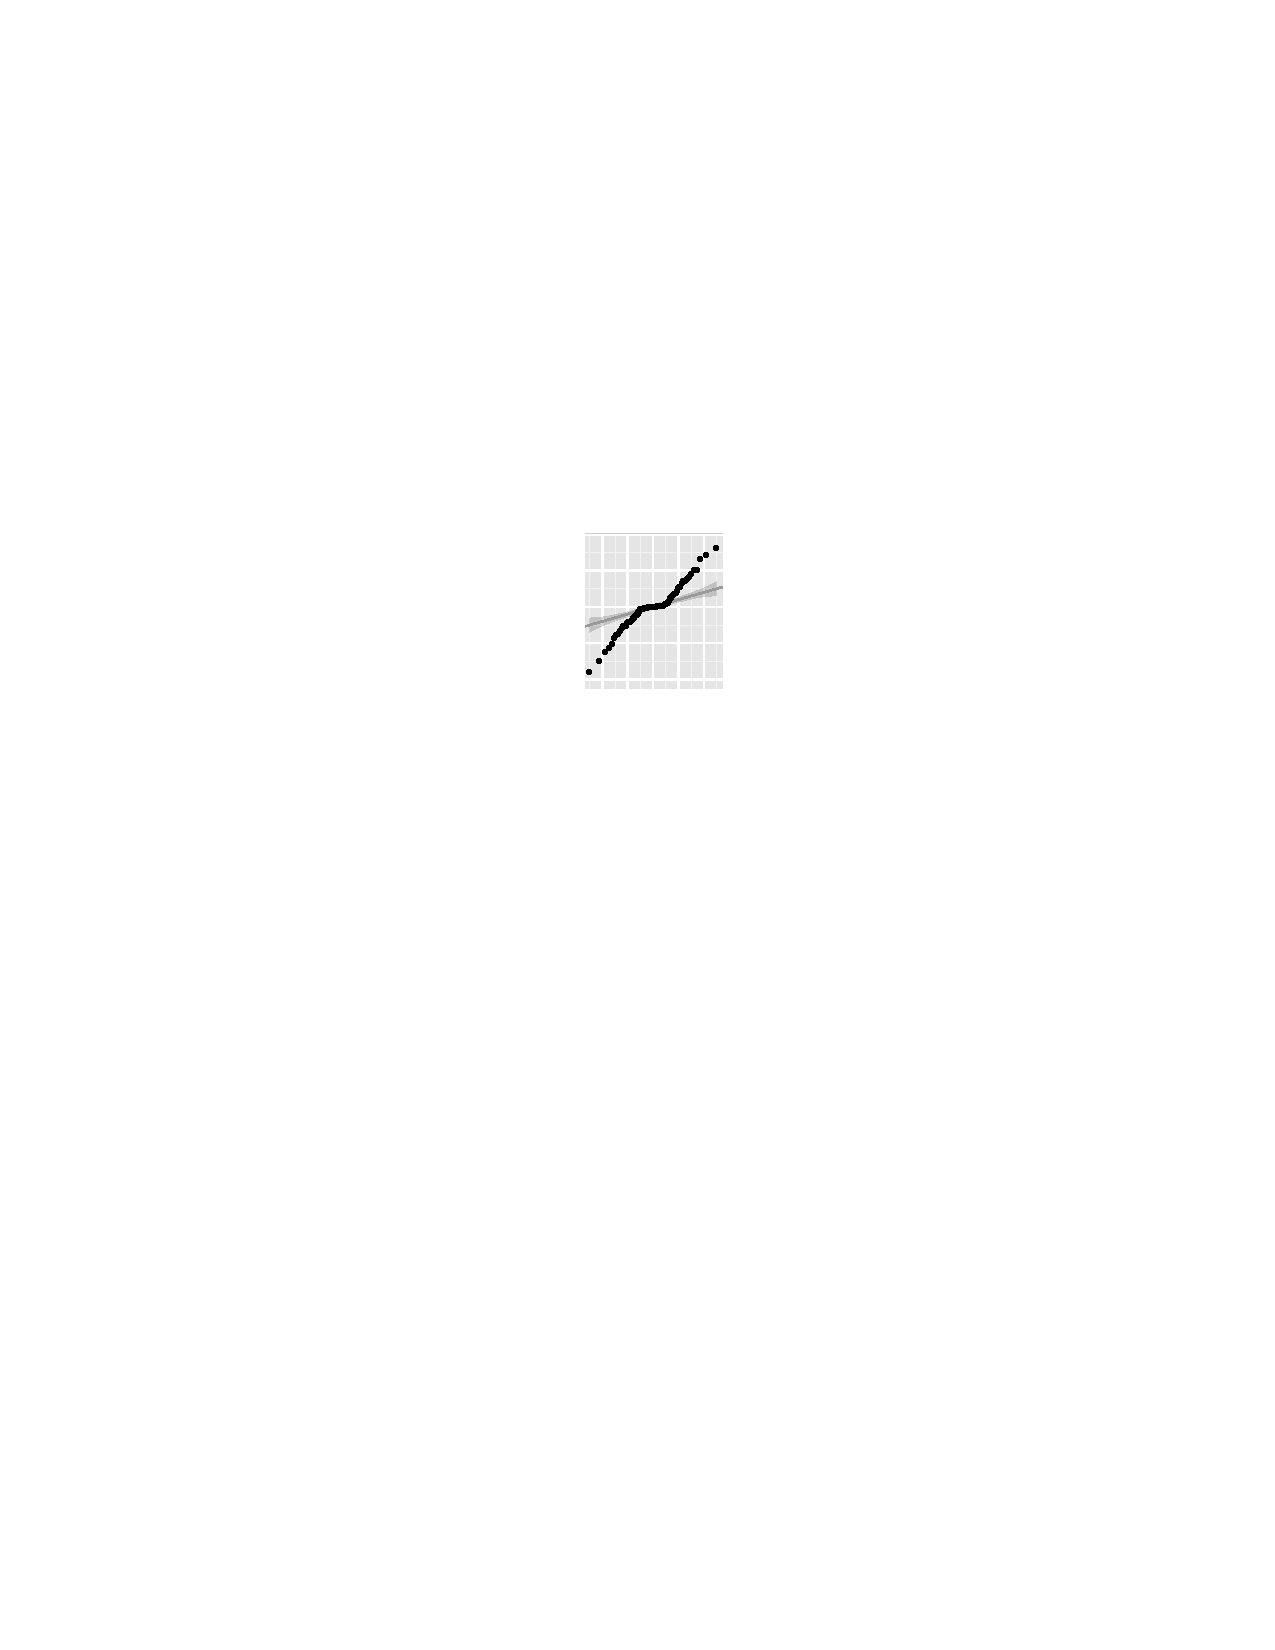
\includegraphics[width=0.22\textwidth]{residual1.pdf}\hfill
\includegraphics[width=0.22\textwidth]{residual2.pdf}\hfill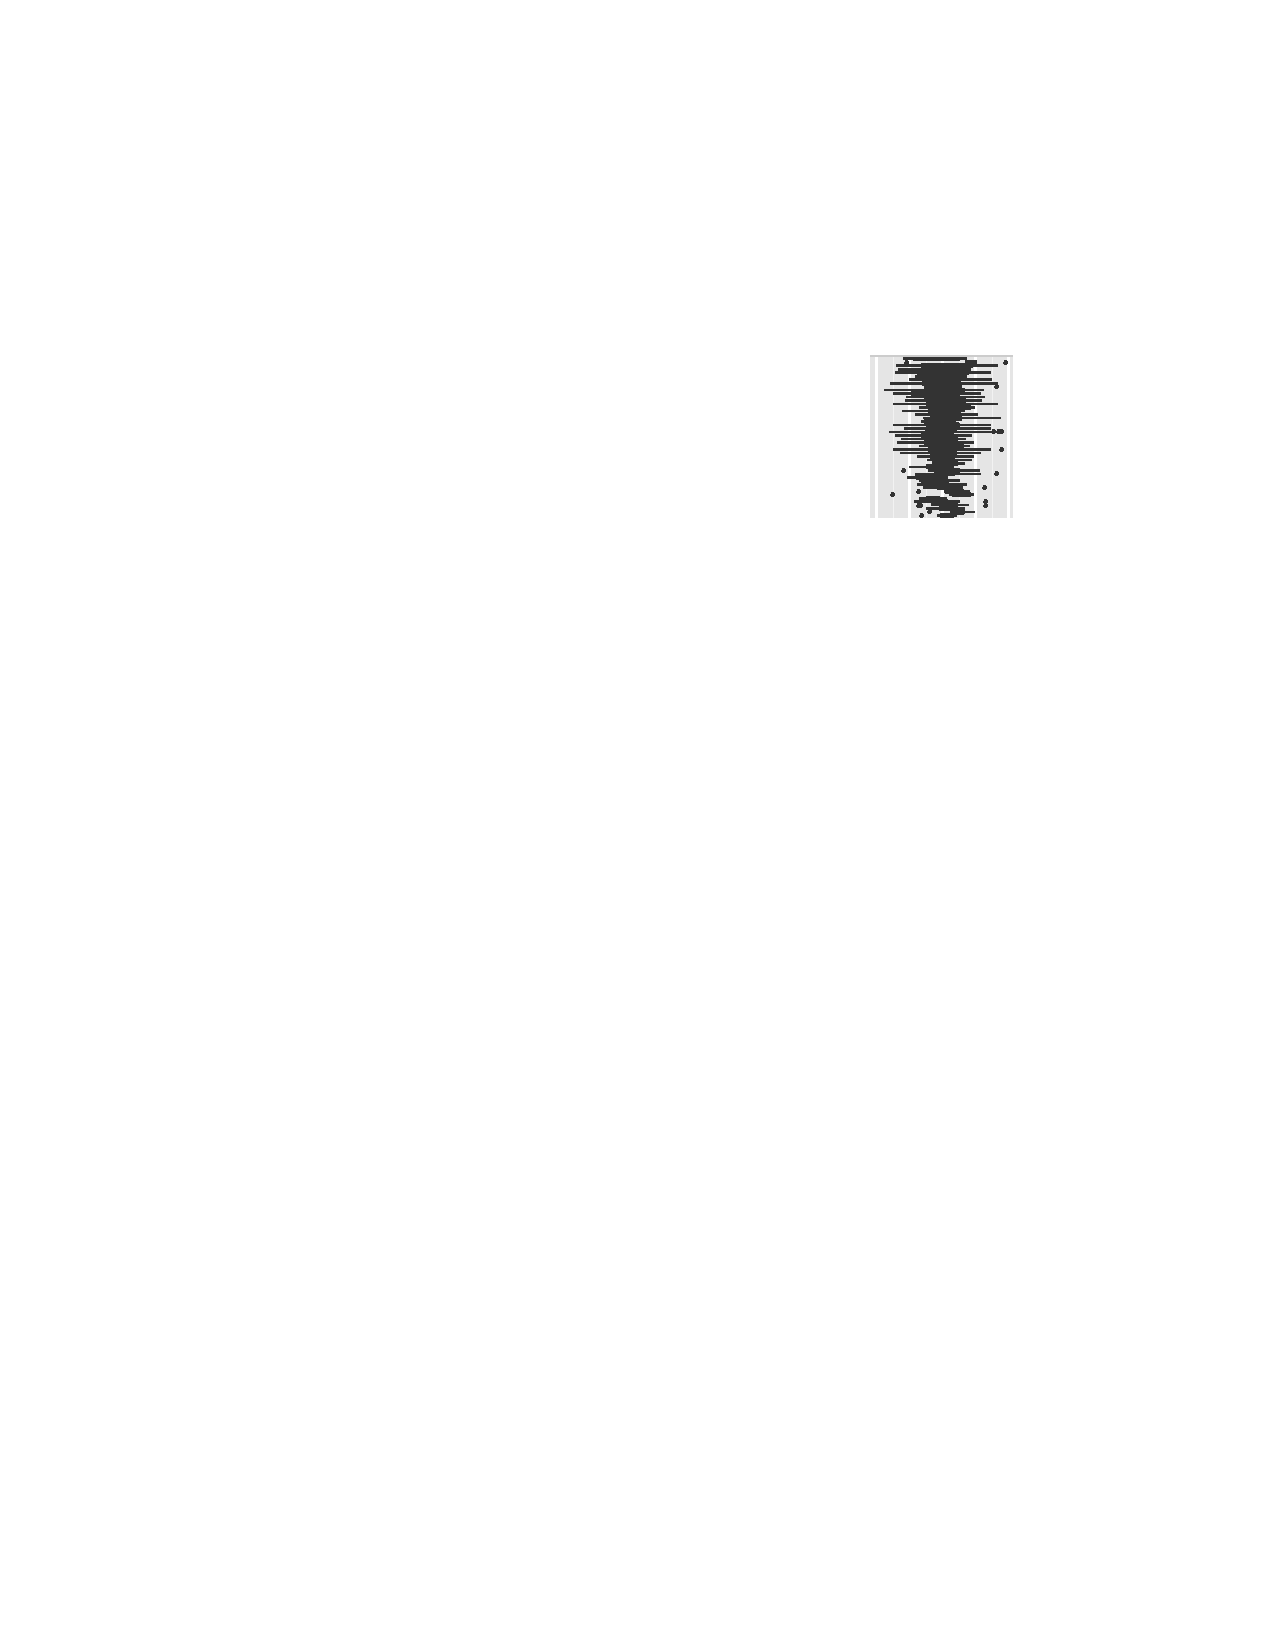
\includegraphics[width=0.22\textwidth]{residual3.pdf}\hfill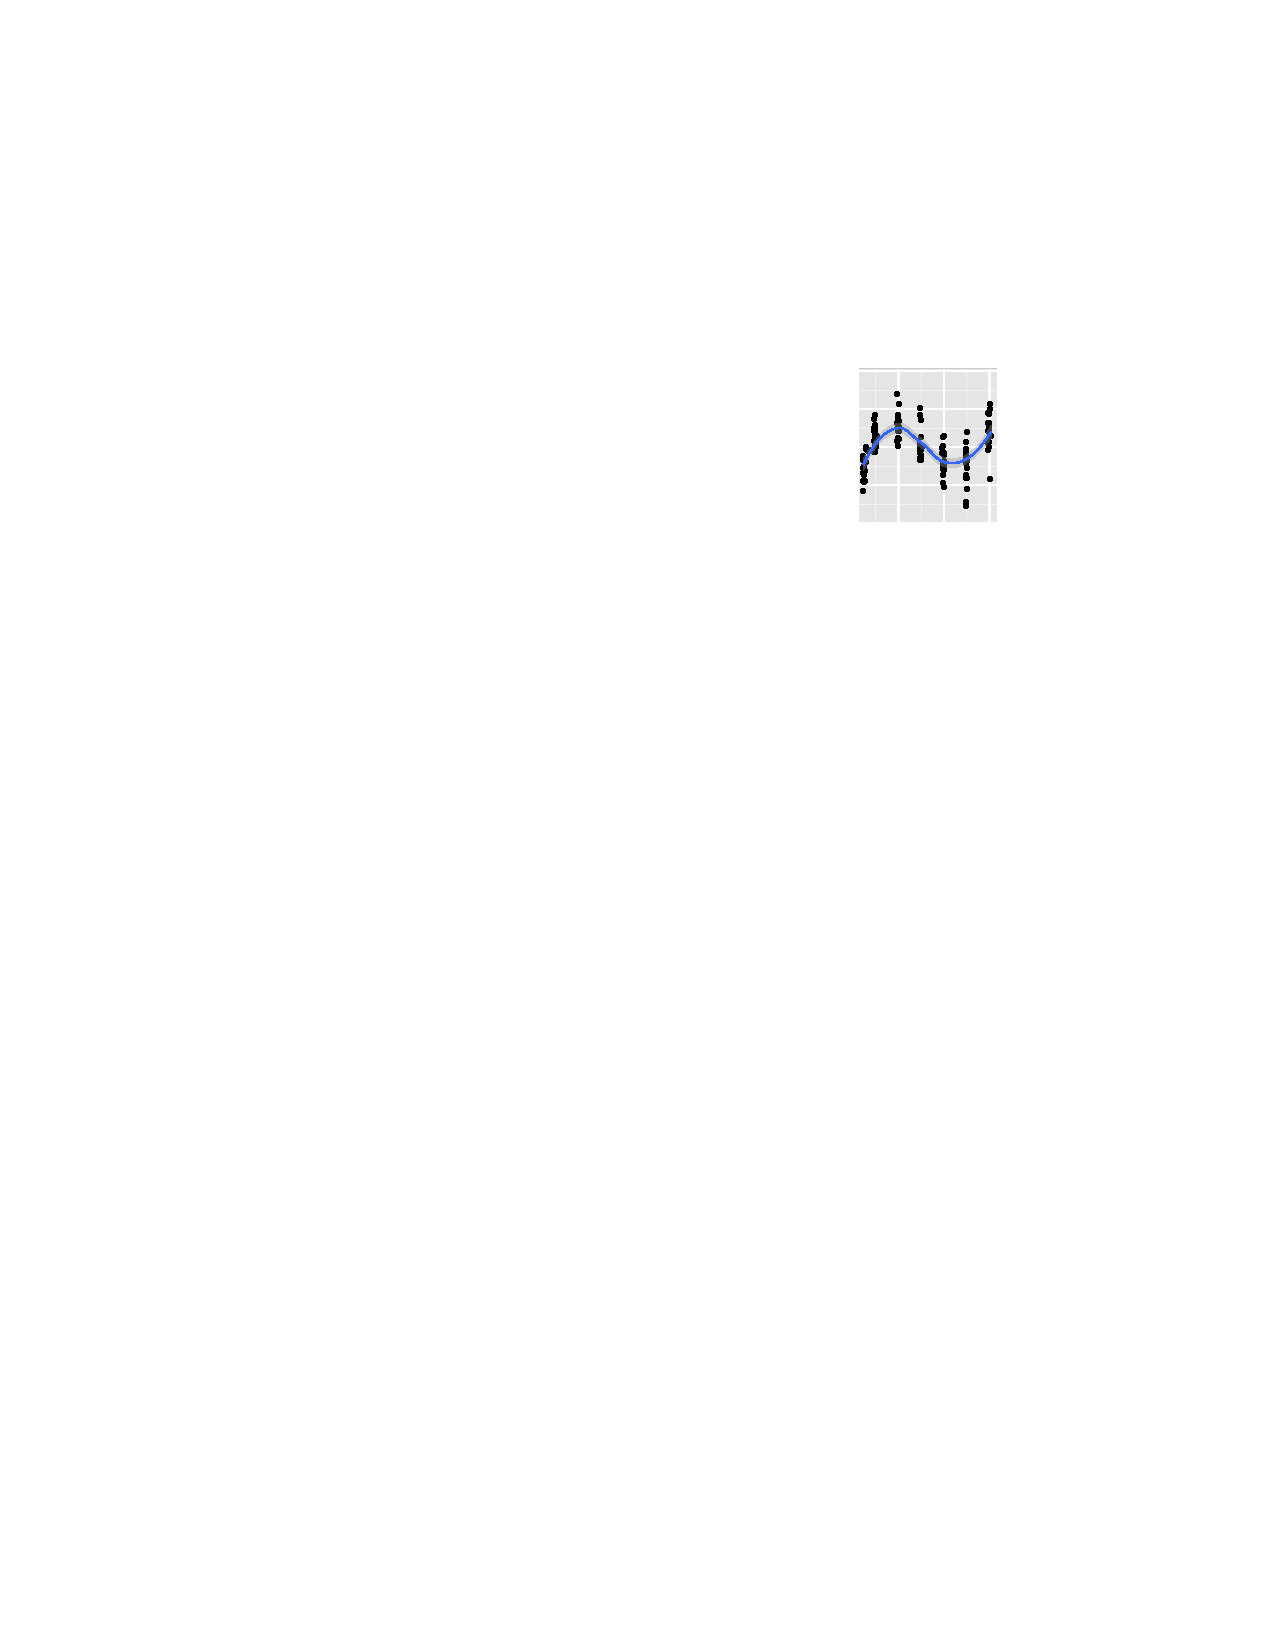
\includegraphics[width=0.22\textwidth]{residual4.pdf}}
%	\caption{\label{fig:motivation2} \dc{Four residual plots from different LME models. Which ones, or all, of these would you consider to indicate structure not captured by the model? (We need something like this right at the start.)}
%	}
%\end{figure}


%The use of random effects models comes at the cost of complicating model exploration and validation. %For example:
%%\hh{In this paper we want to address some of these situations and offer validated graphical diagnostics as solutions:}
%Problems addressed in the paper include:
%
%
%\begin{enumerate}
%\item {\em Model selection:}
%\begin{enumerate}
%\item {\em \al{Assessment of asymptotic distributions}:} Test statistics used for model selection and validation rely on asymptotic reference distributions which often perform poorly in finite sample situations. 
%For example, the \al{unconditional} empirical distribution of the predicted random effects  does not resemble the theoretical distribution unless strong assumptions are met \citep[Theorem 3.2 and Lemma 3.1]{Jiang:1998vt}. In many finite sample situations these assumptions do not hold, making conventional use of Q-Q plots and tests of the empirical distribution function ineffective for distributional assessment \cite[see the supplement of][for supporting simulation results]{adam}.
%
%\item {\em Boundary issues  in the comparison of nested models: } 
%When evaluating the significance of terms in the random effects structure, the likelihood ratio test statistic does not have the usual $\chi^2$ reference distribution if we are testing whether a variance component lies on the boundary of the parameter space. This results in tests for the random effects that tend to be conservative.
%%\cite{Stram:1994wd} argue that using the usual $\chi^2$ reference distribution leads to conservative results, and suggest using a 50:50 mixture of $\chi^2_q$ and $\chi^2_{q+1}$ when testing $q$ versus $q + 1$ random effects; however, this adjustment is not successful in all cases.}
%
%%\item[Incomparability  of nested models due to estimation procedure: ]
%% Comparison of nested models with different fixed effects not possible with REML estimation, too liberal for ML. 
%\end{enumerate}
%
%
%\item {\em Model checking:} Residual plots might display noticeable patterns that are artifacts of both the data structure and the model estimation procedure rather than indications of lack of fit. 
%This problem is especially pronounced for  scatterplots comparing predicted random effects. Such plots can display points falling along a line that is oriented in conflict with the estimated correlation between the random effects \cite[see][for an example]{Morrell:2000ve}. 
%%\hhnote{XXX I'm not quite sure how that would look like}.  
%%\alnote{This would look like a scatterplot with the slope oriented in the wrong direction (i.e., in conflict with the estimated correlation from ML or REML). I haven't encountered this in practice, but it is what Morrell and Brant talk about.}
%Additionally,  plots of the error terms often exhibit patterns that appear to be indicative of heteroscedasticity, but are merely consequences of data imbalances or sparsity.
%
%\end{enumerate}
%
%The above issues are well-known, and in special circumstances adjustments to the methodology have been proposed. For example, \cite{Stram:1994wd} suggest using a 50:50 mixture of $\chi^2_q$ and $\chi^2_{q+1}$ when testing $q$ versus $q + 1$ random effects; however, this adjustment is not successful in all cases.  \cite{Lange:1989uu} suggest using weighted Q-Q plots to assess the distributional assumptions made on the random effects. This approach is effective in settings where the residual variance, $\sigma^2$, is small relative to the variance components for the random effects, but breaks down when this is not the case \citep{adam}.
% 
%
%%\hh{Why are you going back to lineups now? - it might be better to shift this sentence back by a couple of paragraphs}
%%Lineups for visual inference heavily rely on the types of residuals defined above. %Next, we compare conventional and visual inference for model selection and validation.
%%Below we discuss methods commonly used to check the validity of the assumptions made on model \eqref{eq:hlm} using the level-1 and -2 residuals.
%
%
%The purpose of this paper is to illustrate the use of visual inference for diagnosing LME model fits, and propose graphical tests that can be broadly used in situations where the assumptions of conventional inferential procedures are violated. This approach harnesses the power of graphical diagnostics and, with the rigor of the visual inference framework, constructs tests that address some of these problems without requiring additional assumptions while providing a unified approach for LME models that  also works  in situations where conventional inference is appropriate.
%% \al{Further, this approach provides a unified testing framework for LME models, even }
%
%
%The remainder of this paper is organized as follows. 
%Section~\ref{sec:vi} provides an introduction to the framework of visual inference and the lineup protocol. Sections~\ref{sec:select} and \ref{sec:checking} expand on the problems encountered in model selection and model checking, respectively, and presents solutions utilizing visual inference. 
%%In Section~\ref{sec:checking} we present graphical tests for model validation. 
%Throughout both sections multiple examples are used, and comparisons between conclusions on model building and fit from the new visual inference approach and existing diagnostic tools are provided. All example data sets are readily available for public use. A short description of each data set can be found in Section~1 of the appendix.
%
%%\alnote{Should we include another pointer to the descriptions of the data sets?}
%%\hhnote{Usually contents of the appendices aren't discussed in the introduction - but we need to extend the description of the paper a little bit more, you're right with that!}
%
%%We also show results of a study investigating the power of three different versions of the familiar Q-Q plot. 
%
%%\todo[inline]{paragraph on the structure of the paper:  next section deals with visual inference in the framework of hierarchical models, and suggests a series of visual tests as alternative to tests that in the classical setting don't work too well because of easily violated assumptions or nature of the setup. Then we will discuss using power to choose specific designs in the evaluation of distributional assumptions in the familiar graphical setting of the Q-Q plots. }
%

\section{Data sets}\label{supp:datasets}
%------------------------------------------------------------------------------------

All of the data sets used in this paper are publicly available: the General Certificate of Secondary Education Exam data set is available in the R package mlmRev \citep{mlmRev}; the Dialyzer data set is available in the R package MEMSS \citep{MEMSS}; all other data sets can be found in the R package HLMdiag \citep{HLMDiag}.

\subsection{General certificate of secondary education exam data}\label{data:GCSE}

We make use of a subset of examination results of 4,065 students nested within 65 inner-London schools discussed by \cite{Goldstein:1993wm}. The original analysis explored school effectiveness as defined by students' performance on the General Certificate of Secondary Education Exam (GCSEE) in both mathematics and English. This exam is taken at the end of compulsory education, typically when students are 16 years old.  To adjust for a student's ability when they began secondary education, the students' scores on the standardized London Reading Test (LRT) and verbal reasoning group (bottom 25\%, middle 50\%, or top 25\%) at age 11 were recorded. Additional information contained in the data set includes student gender, school gender, and the average LRT intake score for each school. 


\subsection{Autism study}\label{data:autism}
%------------------------------------------------------------------------------------
%\alnote{I need to pare this down.}
%Autism is a developmental disorder typically characterized by impaired communication and social skills, but there is relatively little consensus on how these abilities or disabilities change over time \citep{Anderson:2007cl, Anderson:2009in}. 
In an effort to better understand changes in verbal and social abilities from childhood to adolescence, \cite{Anderson:2007cl, Anderson:2009in} carried out a prospective longitudinal study following 214 children between the ages of 2 and 13 who had been diagnosed with either autism spectrum disorder or non-spectrum developmental delays at age 2. The Vineland Adaptive Behavior Interview survey was used to assess each child's interpersonal relationships, play time activities, and coping skills, 
%This survey is completed by the parents. 
from which the Vineland Socialization Age Equivalent (VSAE) was computed as an overall measure of a child's social skills. Additionally, expressive language development at age 2 was assessed using the Sequenced Inventory of Communication Development (SICD) and the children were classified into three groups (high, medium, or low). Assessments were made on the children at ages 2, 3, 5, 9, and 13, however, not all children were assessed at each age. Additional information collected on each child includes: gender, race (white or non-white), and initial diagnosis at age 2 (autism, pervasive development disorder (pdd), or non-spectrum). We restricted attention to models concerned with the changes in social skills for subjects diagnosed with autism spectrum disorder having complete data. This results in a reduced data set of 155 children. For more detailed analyses we refer the reader to \cite{Anderson:2007cl, Anderson:2009in}.

\subsection{Methylprednisolone study}\label{data:ahd}
%------------------------------------------------------------------------------------

\cite{Carithers:1989} conducted a four week longitudinal study to investigate the effectiveness of methylprednisolone to treat patients with severe alcoholic hepatitis. The researchers randomly assigned 66 patients to receive either methylprednisolone (35 patients) or a placebo (31 patients). Over the study duration, each subject's serum bilirubin levels (in $\mu$mol/L) were measured each week, with the first measurement taken at the start of the study (week 0).

\subsection{Dialyzer study}\label{data:dialyzer}
%------------------------------------------------------------------------------------

\cite{Vonesh:1992us} describe a study characterizing the water transportation characteristics of 20 high flux membrane dialyzers, which were introduced to reduce the time a patient spends on hemodialysis. The 20 dialyzers were studied \emph{in vitro} using bovine blood at flow rates of either 200 or 300 ml/min, and the ultrafiltration rate (ml/hr) for each dialyzer was measured at seven transmembrane pressures (in mmHg). \cite{Vonesh:1992us} use nonlinear mixed-effects models to analyze these data; however, they can be modeled using polynomials in the linear mixed-effects framework \citep[see][Section 9.5]{Littell:2006}.

\subsection{Radon study}\label{data:radon}
%------------------------------------------------------------------------------------

The data consist of a stratified random sample of 919 owner-occupied homes in 85 counties in Minnesota. For each home, a radon measurement was recorded (in log $pCi/L$, i.e., log picoCuries per liter) as well as a binary variable indicating whether the measurement was taken in the basement (0) or a higher level (1). Additionally, the average soil uranium content for each county was available. The number of homes within each county varies greatly between counties ranging from one home to 116 homes, with 50\% of counties having measurements from between 3 and 10 homes. \cite{Gelman:2006ue} suggest a simple hierarchical model allowing for a random intercept for each county and a random slope for floor level. This is the model from which we simulate predicted random effects.

%------------------------------------------------------------------------------------
\section{Experimental Setup and Results}\label{study}
%------------------------------------------------------------------------------------
\subsection{Experimental Setup and Calculation of $p$-values}\label{sec:pvalues}
For each of the lineup designs described in the paper we constructed five replicates consisting of the same data plot and different sets of nineteen null plots for a total of 75 different lineups. These were evaluated by 487 participants in altogether 4927 evaluations. For each lineup, observers were instructed to identify the plot  most different from the set and asked what feature led them to their choice. 
These choices came in the form of four suggestions (in checkboxes) and one text box for a free-form answer. For each lineup the time taken to answer was recorded and  observers were asked for their confidence level (on a scale from 1=weak to 5=high). Observers were also asked to provide their demographics: age category, gender,  education range, and geographic location (from parts of the ip address). 

The results of the evaluations for all lineups  are displayed in Table~\ref{tab:results} and the observers' reasons for identifying plots are summarized in Table~\ref{tab:reasons}. 
The significances in Table~\ref{tab:results} are based on the number of evaluations and the number of times that the data plot was identified. For that, we the introduce the random variable $Y$ as the  number of evaluations of a lineup in which the observer identifies the data plot. Assume that the lineup has size $m=20$, and it is shown to a total of $K$ independent observers.  Then $Y$ has a Visual distribution $V_{K, m, s=3}$ as defined in \citet{hofmann:2015},
where $s$ delineates scenario III---i.e., the same lineup is shown to all $K$ observers. The $p$-values in Table~\ref{tab:results} for each of the five replicates are calculated this way.
For the overall $p$-value, we use a simulation based approach to combine the five results. Treating the number of evaluations $(K_1, ..., K_5)$ as fixed, we simulate assessments of lineups without signal as follows: we assume that the signal in a plot is complementary to its $p$-value, which is i.i.d. $U[0,1]$ under the null hypothesis. We further assume that the probability an observer picks a  plot  is allocated proportionally to its signal. For each ``data plot'' we create five sets of null plots to be evaluated simultaneously $(K_1, ..., K_5)$ times.  
$p$-values are then based on a comparison of the sum of data picks from  five no-signal lineups and  the observed number of data picks from the actual lineups. The column on the right of Table~\ref{tab:results} shows $p$-values based on $10^5$ simulation runs.


%How did we get the data? Some information on Amazon Turk, and setup of experiments. 

%\hhnote{Data collected for each response: time taken, answer(s), confidence level and reason for choice - four suggestions in form of check boxes, one text box;
%data collected on each participant: gender, age group, education level, geography (from ip address), nickname to match responses from the same individual. }


%%------------------------------------------------------------------------------------
%\subsection{Discussion of study results} % and participants' demographics}
%%------------------------------------------------------------------------------------
%
%%All of the lineups discussed in this paper (and the two presented in Appendix~\ref{app:morelineups}) were evaluated using Amazon MTurk. All  lineups were evaluated in the same study, which we describe below.
%
%%For each of the ten lineups, five replications were constructed for a total of 50 lineups. The replications for the lineup in Figure~\ref{fig:qqlineup-t} were created by different simulations, while the replications for the remaining lineups were created by shuffling the location of the true plot and exchanging the null plots for additional simulations under the null model. For each lineup, observers were instructed to identify the plot that is most different and asked what feature led them to their choice. Overall the study was comprised of  334 participants who made 3441 evaluations. 
%
%The results show that for all but the Q-Q plots of the random slopes, enough observers identified the true plot so that we reject the null hypotheses that the data are consistent with what is expected under the null model. For the Q-Q plot of the random slopes generated by a $t$ distribution, three of the five replicates resulted in a rejection of the null hypothesis of normality. The variability in the results is explained by different ``true'' plots being simulated for each replicate. 



%\hhnote{I'm not sure how much more detail we can give here - we're in the process of writing up the exact distribution, but the vinference package on my github site already allows for a calculation of the corrected $p$-values.}
%\alnote{Can we cite the R package? Having a citation might help with this.}
%
%\hhnote{Only three out of five replicates are providing significant results against the null hypothesis.}
%
%\hhnote{Explain how we deal with five $p$-values from five lineups with the same data and different null sets }


%\hh{There are five different null sets for each data set. Throughout the paper we show lineups for the first replicate. In all of the lineups with the exception of figure~\ref{fig:qqlineup-1} observers are identifying the data plot to a degree that we have to reject the null hypotheses of the data being consistent with the null model. }
%\hh{For the radon t ranef example we have actually five different samples from a $t$ distribution in the lineups - that explains the much larger variability between the results. }

% latex table generated in R 3.0.1 by xtable 1.7-1 package
% Tue Jun  4 23:00:42 2013
\begin{table}[ht]
\centering
\caption{\label{tab:results} Overview of all lineup evaluations. Ratios comparing the number correct to the total number of evaluations are shown.  $p$-values and significances are based on the calculations as described in Section~\ref{sec:pvalues}.
} 
\begin{tabular}{Mrrlrlrlrlrlc}
  \hline
&  & \multicolumn{9}{c}{Replicate} && Overall \\ \cline{3-12} 
\multicolumn{2}{c}{Lineup} & 1 & & 2 && 3 && 4 && 5 && $p$-values\\ 
  \hline
  

\includegraphics[width=0.05\textwidth]{examfanned-icon}&  fig.~1 &   10/68 & \hspace{-0.1in}* & 7/65 & \hspace{-0.1in}  & 8/61 & \hspace{-0.1in}. & 13/61 & \hspace{-0.1in}*** & 6/66 & \hspace{-0.1in}  & 0.0022 \\ 
%
\includegraphics[width=0.05\textwidth]{examfanned-icon}&  fig.~1 & 11/73&\hspace{-0.1in}* & 7/70&\hspace{-0.1in} & 9/65&\hspace{-0.1in}*& 13/66&\hspace{-0.1in}** & 7/72&\hspace{-0.1in} & 0.0001\\ 
 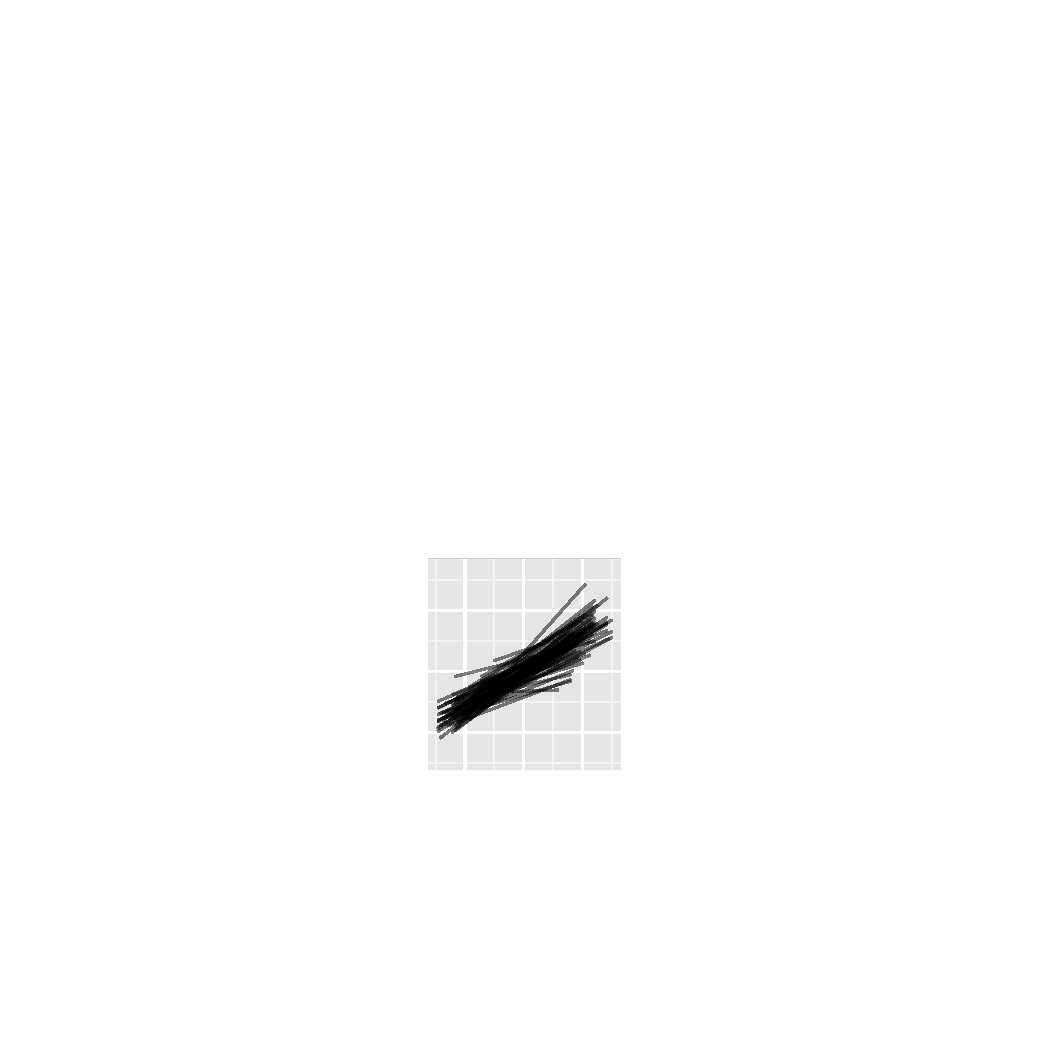
\includegraphics[width=0.05\textwidth]{exam-with-slope-icon} & fig.~3 & 0/64 & \hspace{-0.1in}  & 7/75 & \hspace{-0.1in}  & 11/76 & \hspace{-0.1in}* & 0/69 & \hspace{-0.1in}  & 0/60 & \hspace{-0.1in} & 0.4202 \\ 
%
%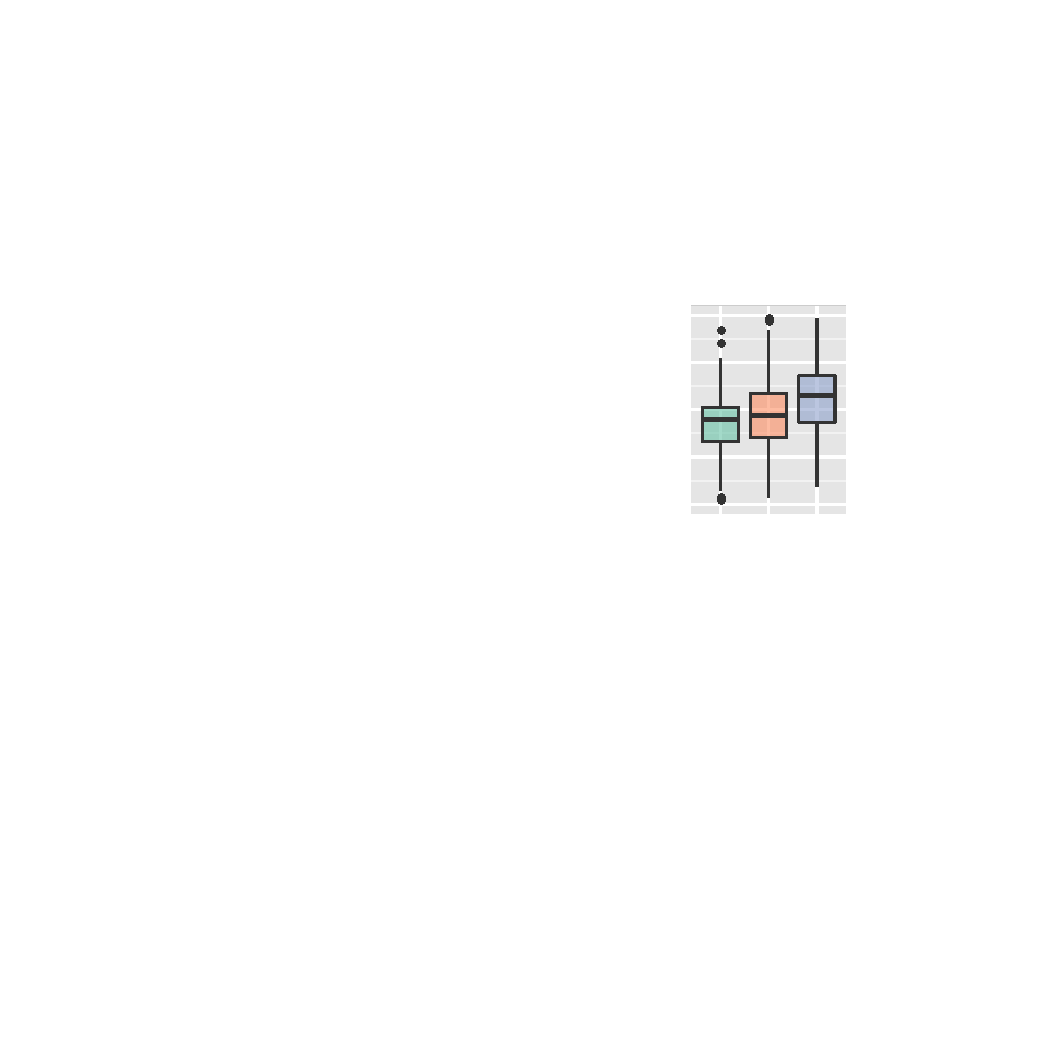
\includegraphics[width=0.05\textwidth]{autism-ordered-icon}&   fig.~2 & 65/74&\hspace{-0.1in}*** & 57/66&\hspace{-0.1in}*** & 62/68&\hspace{-0.1in}*** & 54/63&\hspace{-0.1in}*** & 66/76&\hspace{-0.1in}*** & $<10^{-5}$\\ 
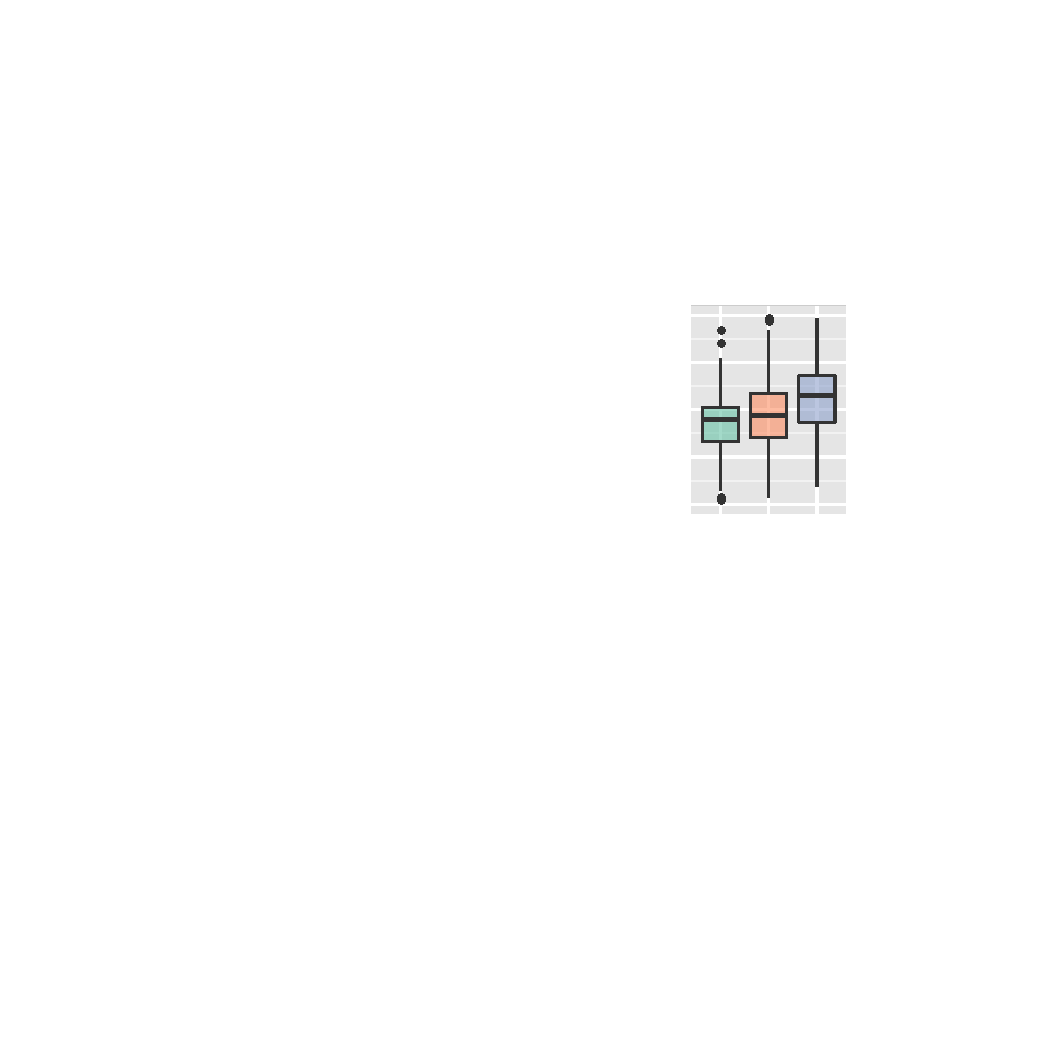
\includegraphics[width=0.05\textwidth]{autism-ordered-icon}&   fig.~2 & 60/68 & \hspace{-0.1in}*** & 51/59 & \hspace{-0.1in}*** & 59/64 & \hspace{-0.1in}*** & 51/60 & \hspace{-0.1in}*** & 62/71 & \hspace{-0.1in}*** & $< 10^{-4}$ \\ 
%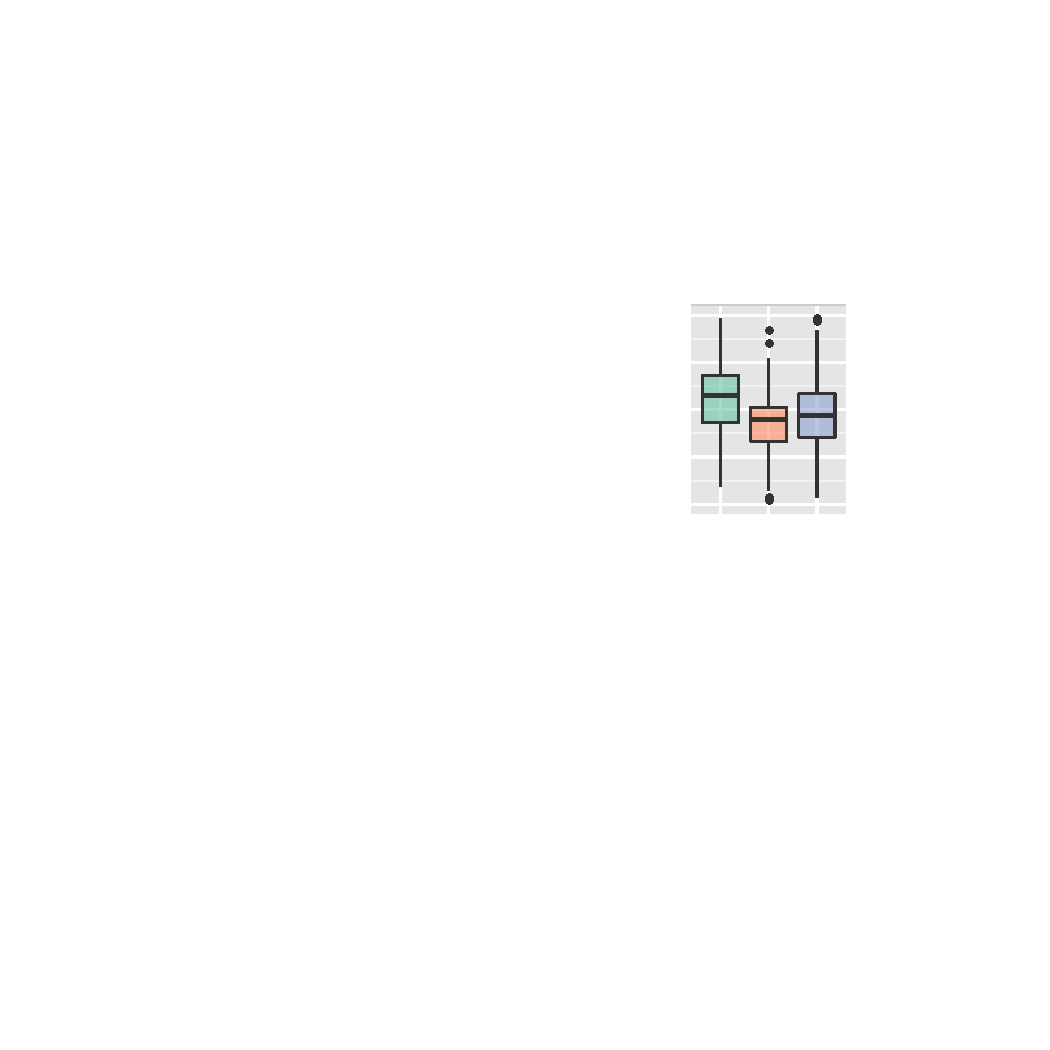
\includegraphics[width=0.05\textwidth]{autism-unordered-icon}&   fig.~\ref{fig:boxplot-unordered} & 52/54&\hspace{-0.1in}***  & 63/76&\hspace{-0.1in}*** & 70/75&\hspace{-0.1in}*** & 59/64&\hspace{-0.1in}*** & 63/70&\hspace{-0.1in}*** & $<10^{-5}$\\ 
 %
 %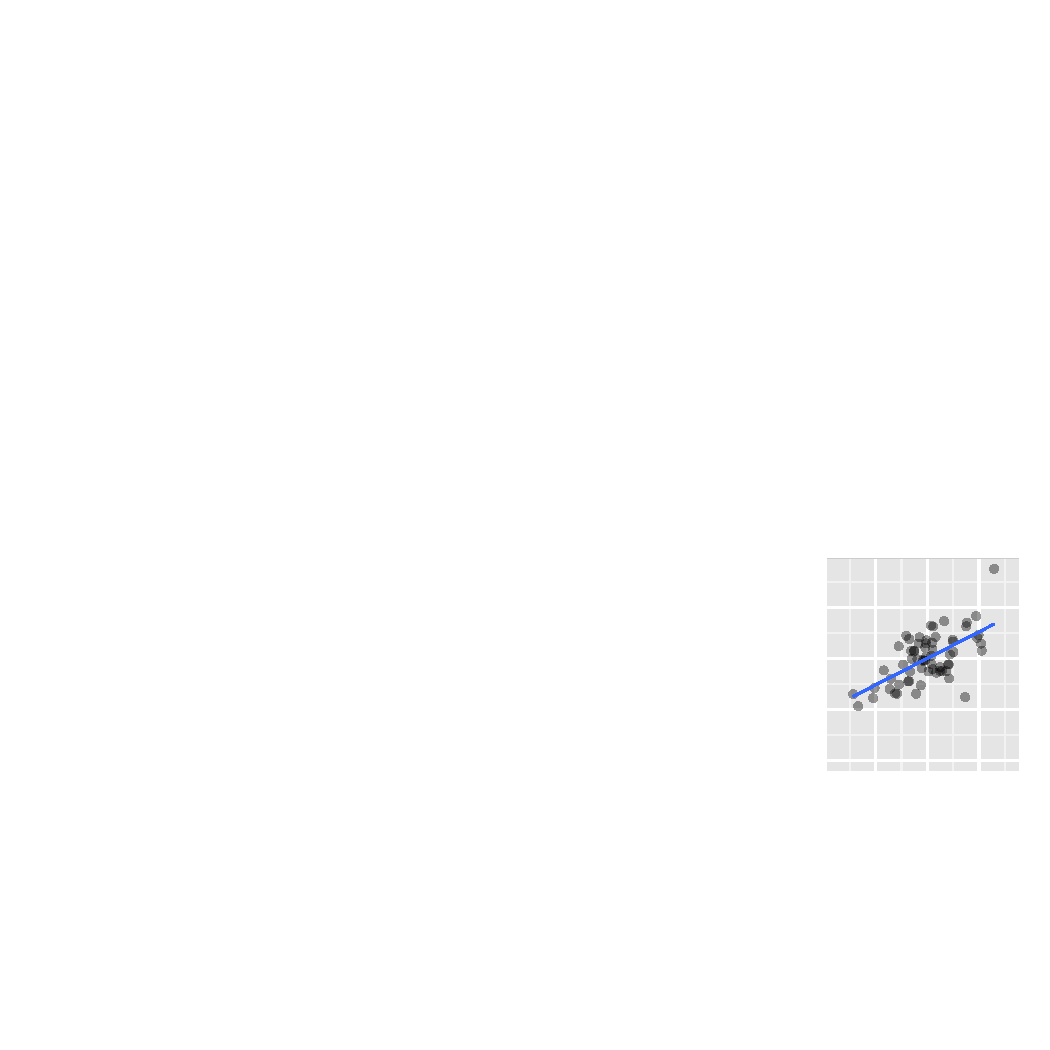
\includegraphics[width=0.05\textwidth]{examcorr-icon}&   fig.~4 & 41/69&\hspace{-0.1in}*** & 62/73&\hspace{-0.1in}*** & 31/64&\hspace{-0.1in}*** & 57/75&\hspace{-0.1in}*** & 55/67&\hspace{-0.1in}*** & $<10^{-5}$\\ 
 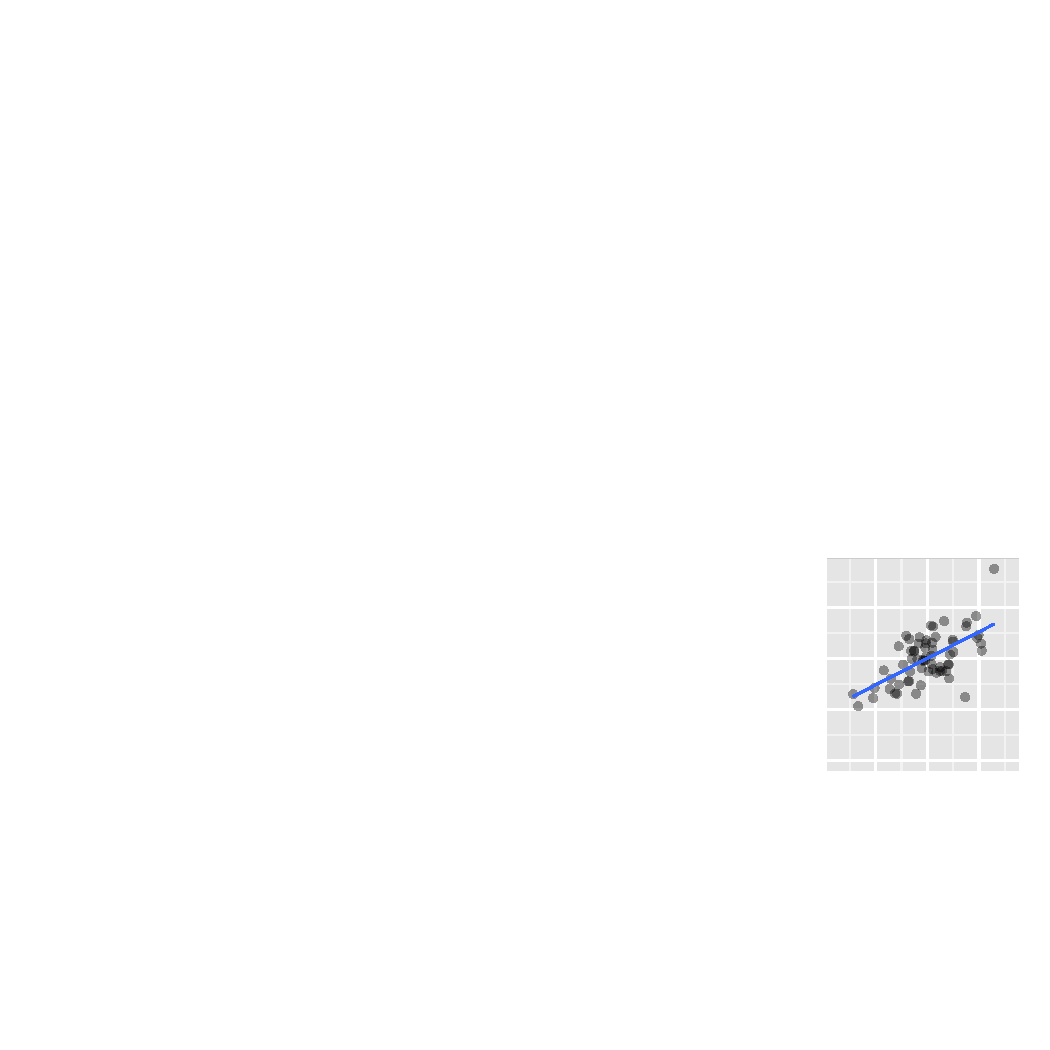
\includegraphics[width=0.05\textwidth]{examcorr-icon}&    fig.~4 & 36/63 & \hspace{-0.1in}*** & 58/69 & \hspace{-0.1in}*** & 30/60 & \hspace{-0.1in}*** & 51/68 & \hspace{-0.1in}*** & 52/63 & \hspace{-0.1in}*** & $< 10^{-4}$ \\ 
 %
%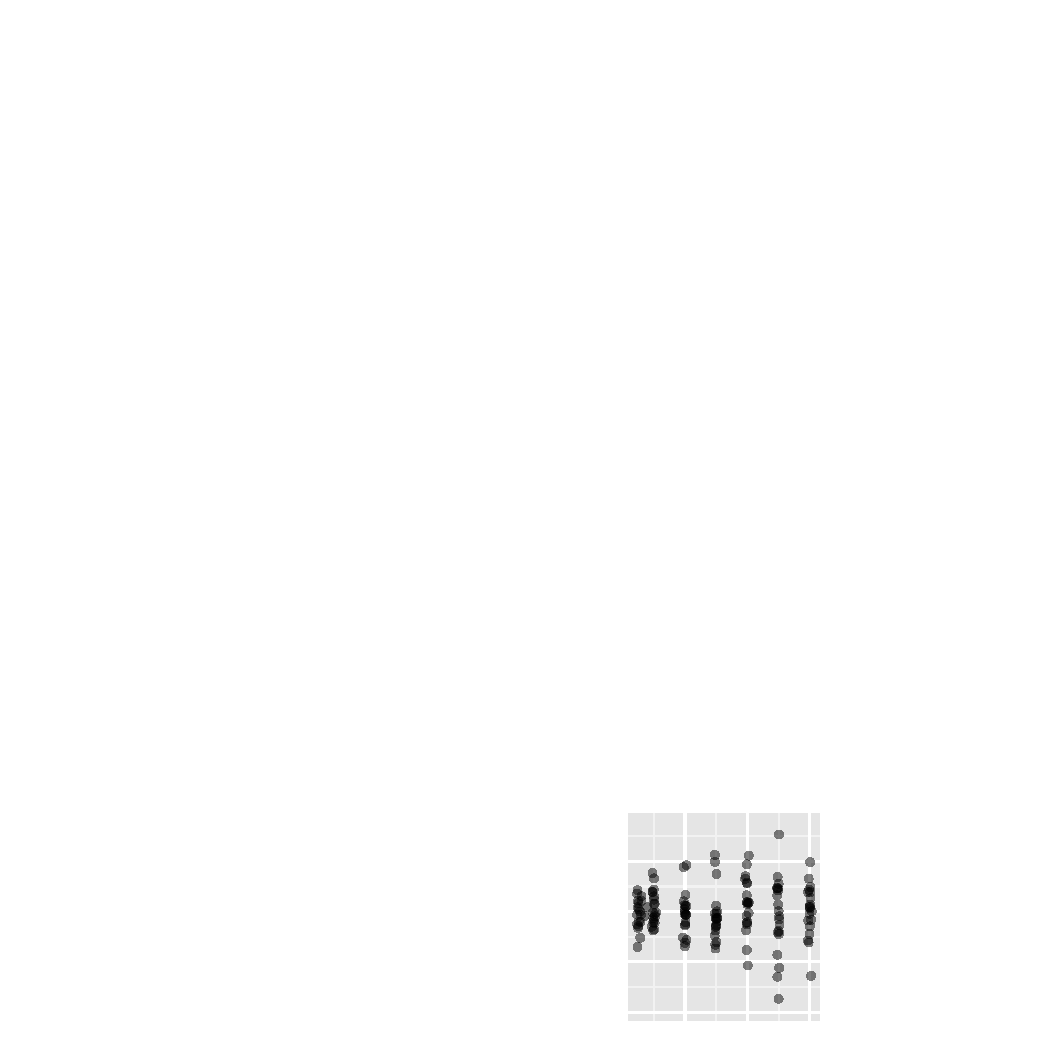
\includegraphics[width=0.05\textwidth]{dialyzerheterogeneous-icon}& fig.~5 & 29/85&\hspace{-0.1in}***  & 10/65&\hspace{-0.1in}* & 24/64&\hspace{-0.1in}*** & 7/60&\hspace{-0.1in}. & 13/72&\hspace{-0.1in}** & $<10^{-5}$\\ 
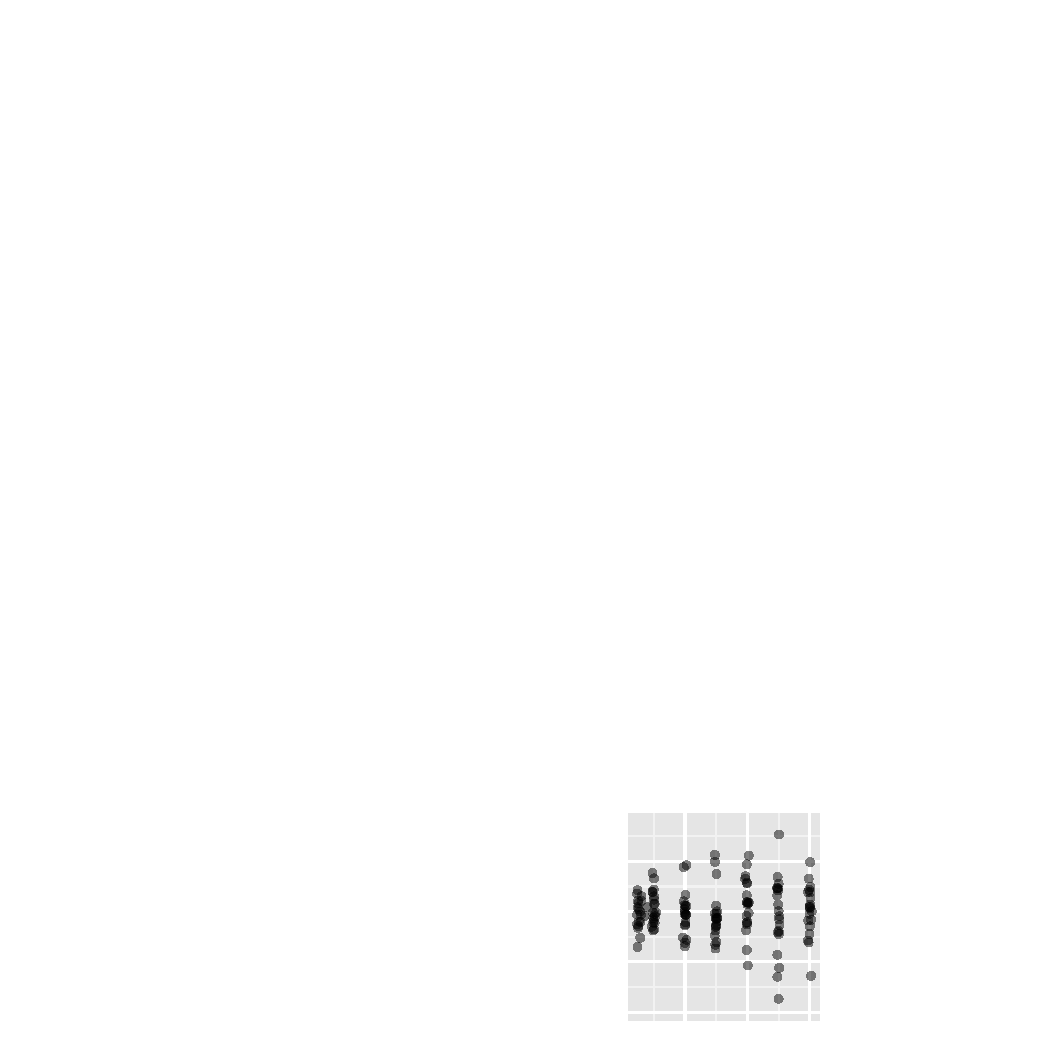
\includegraphics[width=0.05\textwidth]{dialyzerheterogeneous-icon}& fig.~5 & 26/80 & \hspace{-0.1in}*** & 9/59 & \hspace{-0.1in}* & 23/60 & \hspace{-0.1in}*** & 7/55 & \hspace{-0.1in}. & 11/69 & \hspace{-0.1in}* & $< 10^{-4}$ \\ 
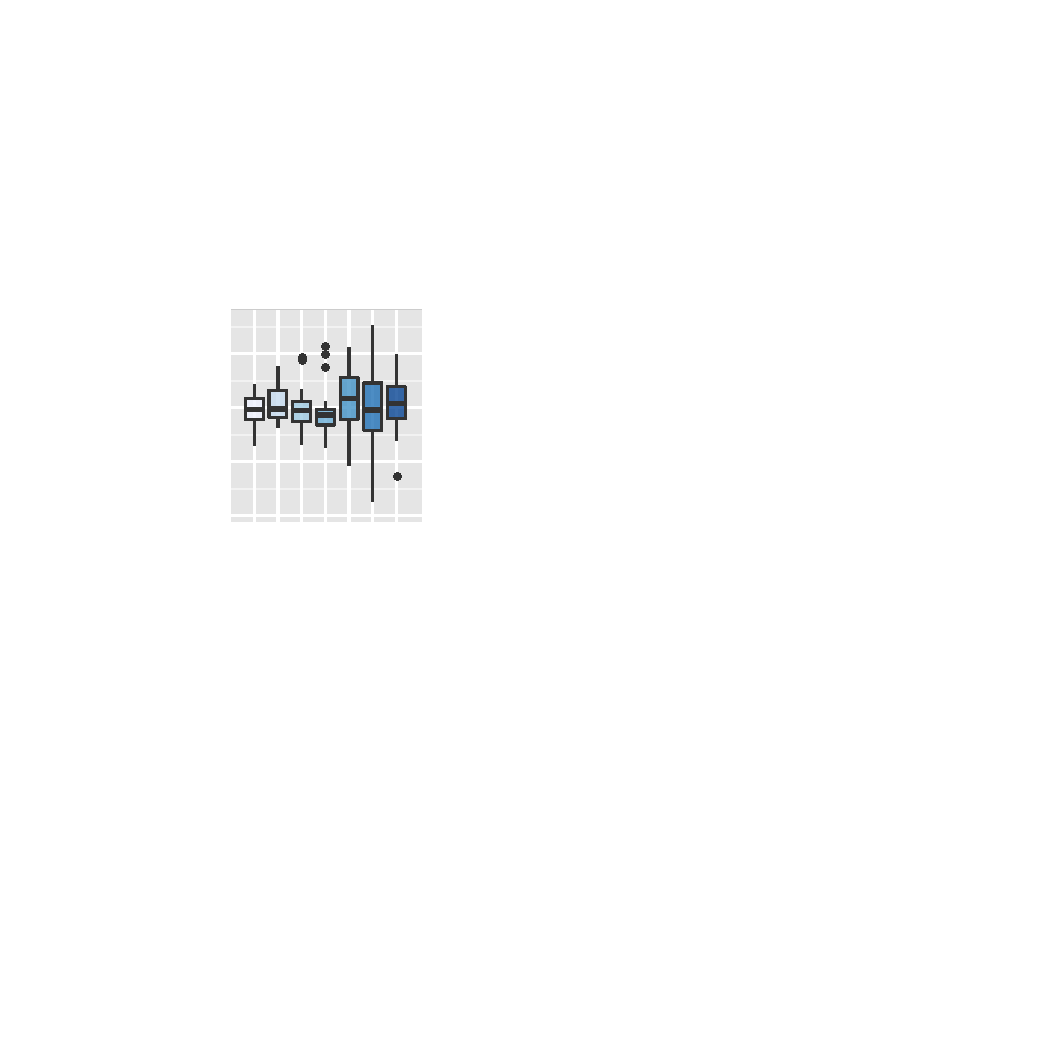
\includegraphics[width=0.05\textwidth]{dialyzerheterogeneous-bp} &  fig.~\ref{fig:constvar2.bp} & 23/70 & \hspace{-0.1in}*** & 9/74 & \hspace{-0.1in}. & 11/62 & \hspace{-0.1in}** & 31/78 & \hspace{-0.1in}*** & 25/61 & \hspace{-0.1in}*** & $<10^{-4}$\\ 
%
%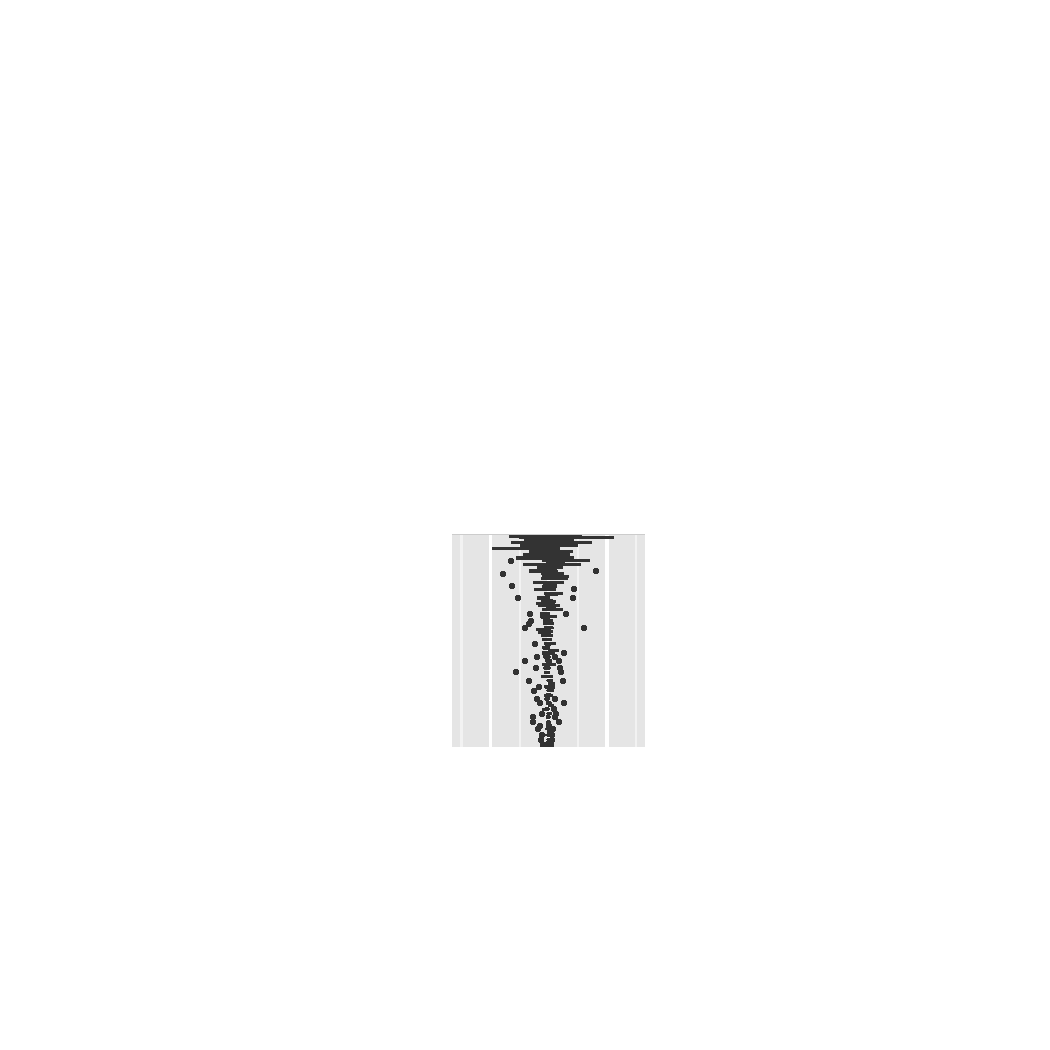
\includegraphics[width=0.05\textwidth]{cyclone-icon}&   fig.~6 & 50/75&\hspace{-0.1in}***  & 44/64&\hspace{-0.1in}*** & 45/68&\hspace{-0.1in}*** & 46/76&\hspace{-0.1in}*** & 50/67&\hspace{-0.1in}*** & $<10^{-5}$\\ 
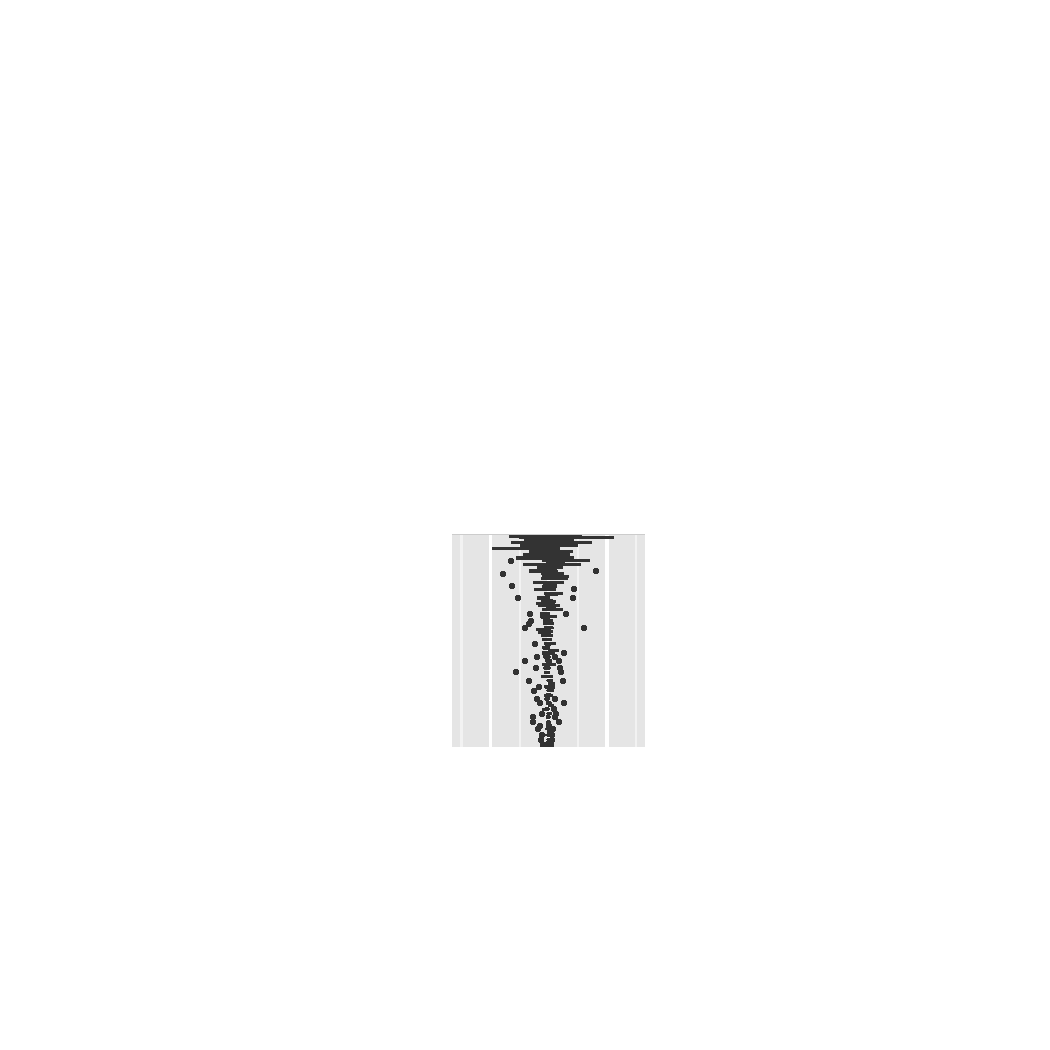
\includegraphics[width=0.05\textwidth]{cyclone-icon}&   fig.~6 & 49/73 & \hspace{-0.1in}*** & 41/59 & \hspace{-0.1in}*** & 41/59 & \hspace{-0.1in}*** & 40/66 & \hspace{-0.1in}*** & 49/65 & \hspace{-0.1in}*** & $< 10^{-4}$ \\ 
%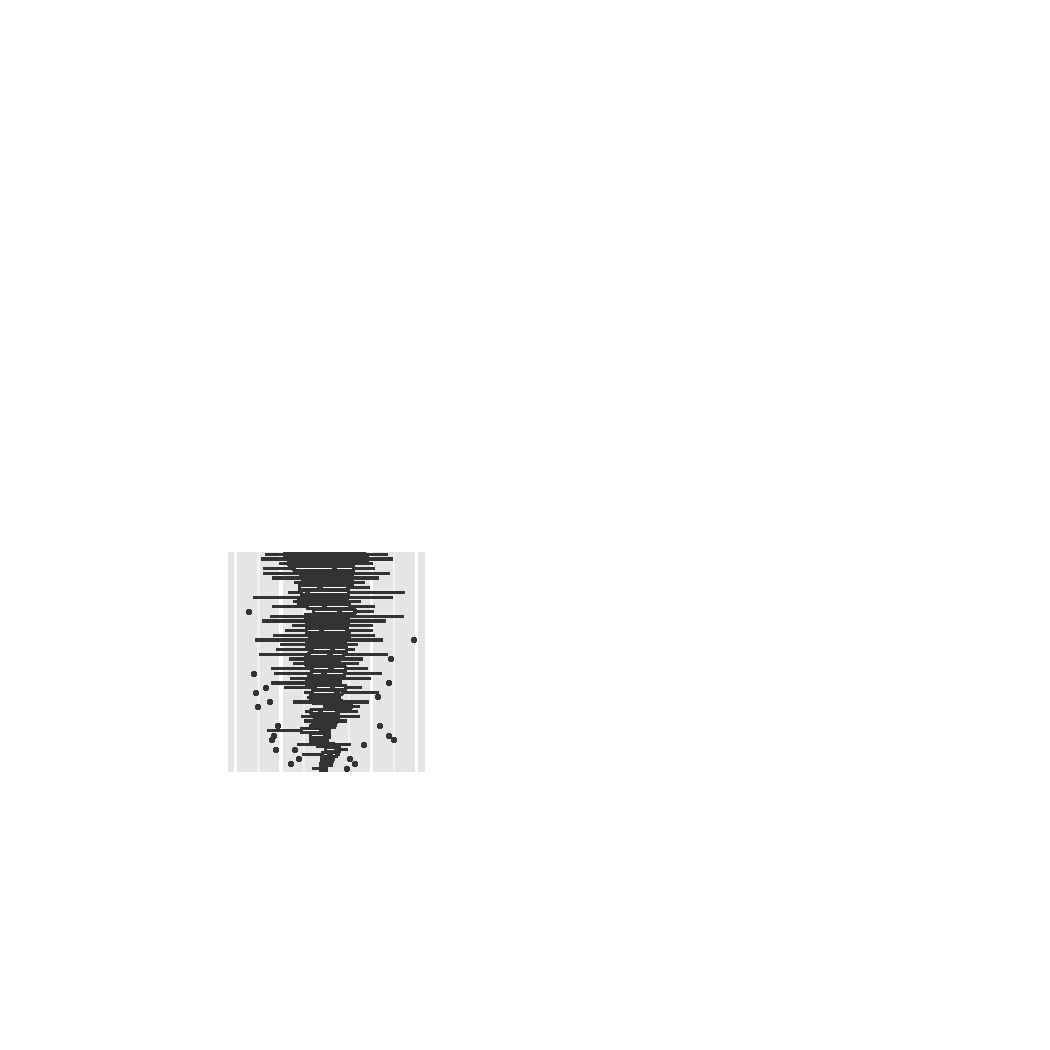
\includegraphics[width=0.05\textwidth]{cyclone-good-icon} & fig.~7  & 1/59 & \hspace{-0.1in}  & 2/79 & \hspace{-0.1in}  & 2/68 & \hspace{-0.1in}  & 4/62 & \hspace{-0.1in}  & 1/73 & \hspace{-0.1in}  & 0.7180\\ 
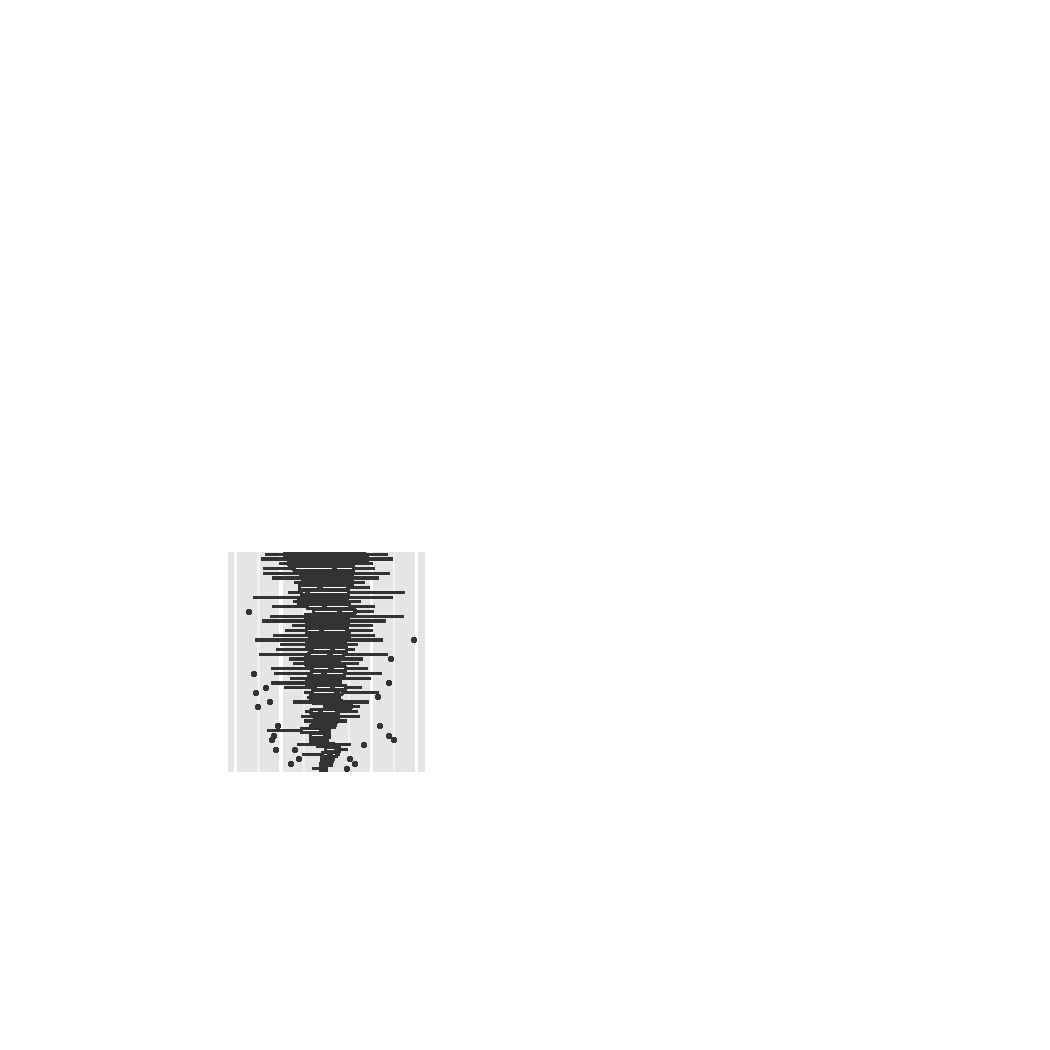
\includegraphics[width=0.05\textwidth]{cyclone-good-icon} & fig.~7  &1/59 & \hspace{-0.1in}  & 2/79 & \hspace{-0.1in}  & 2/68 & \hspace{-0.1in}  & 4/62 & \hspace{-0.1in}  & 1/72 & \hspace{-0.1in}  & 0.6567 \\ 
%
%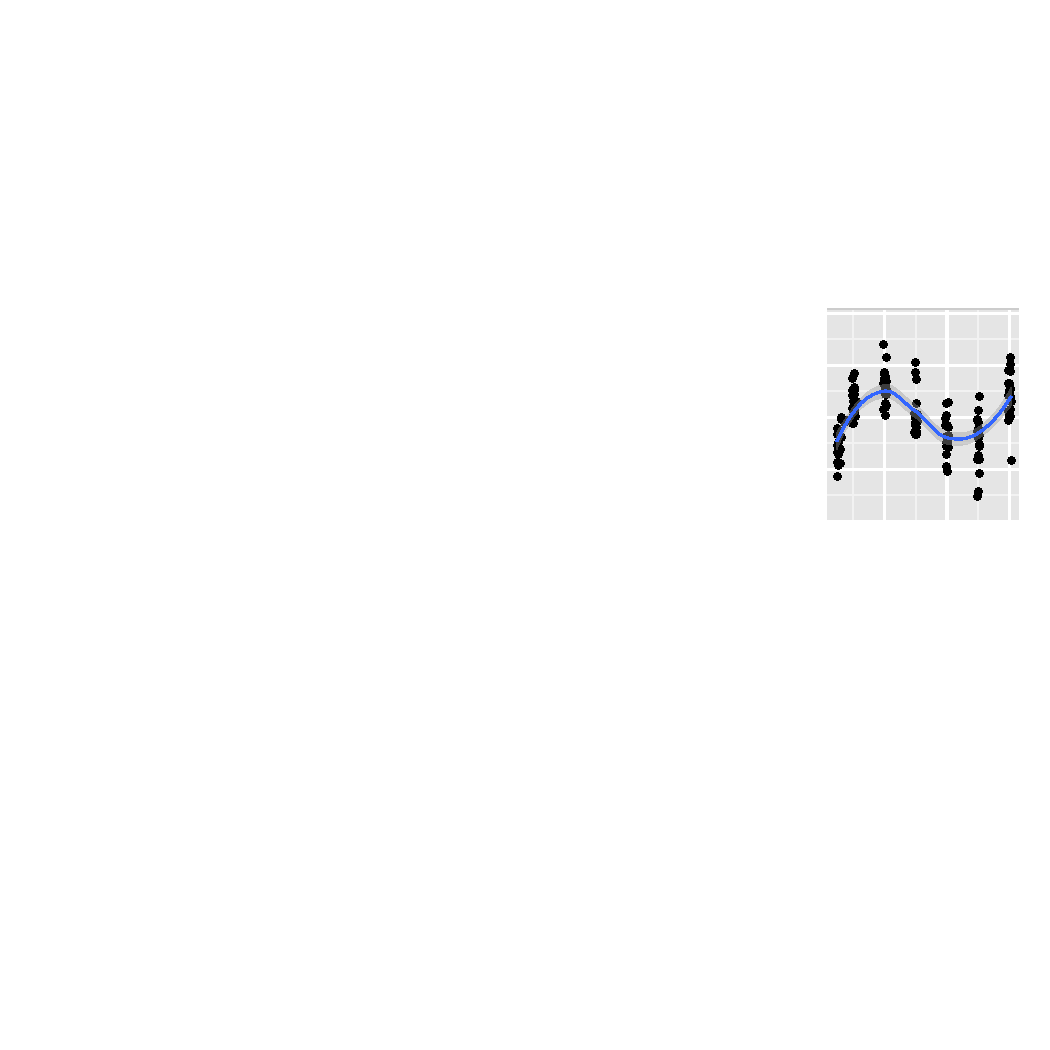
\includegraphics[width=0.05\textwidth]{dialyzernonlinear-icon}&   fig.~8& 60/63&\hspace{-0.1in}***  & 62/64&\hspace{-0.1in}*** & 57/60&\hspace{-0.1in}*** & 84/88&\hspace{-0.1in}*** & 66/69&\hspace{-0.1in}*** & $<10^{-5}$\\ 
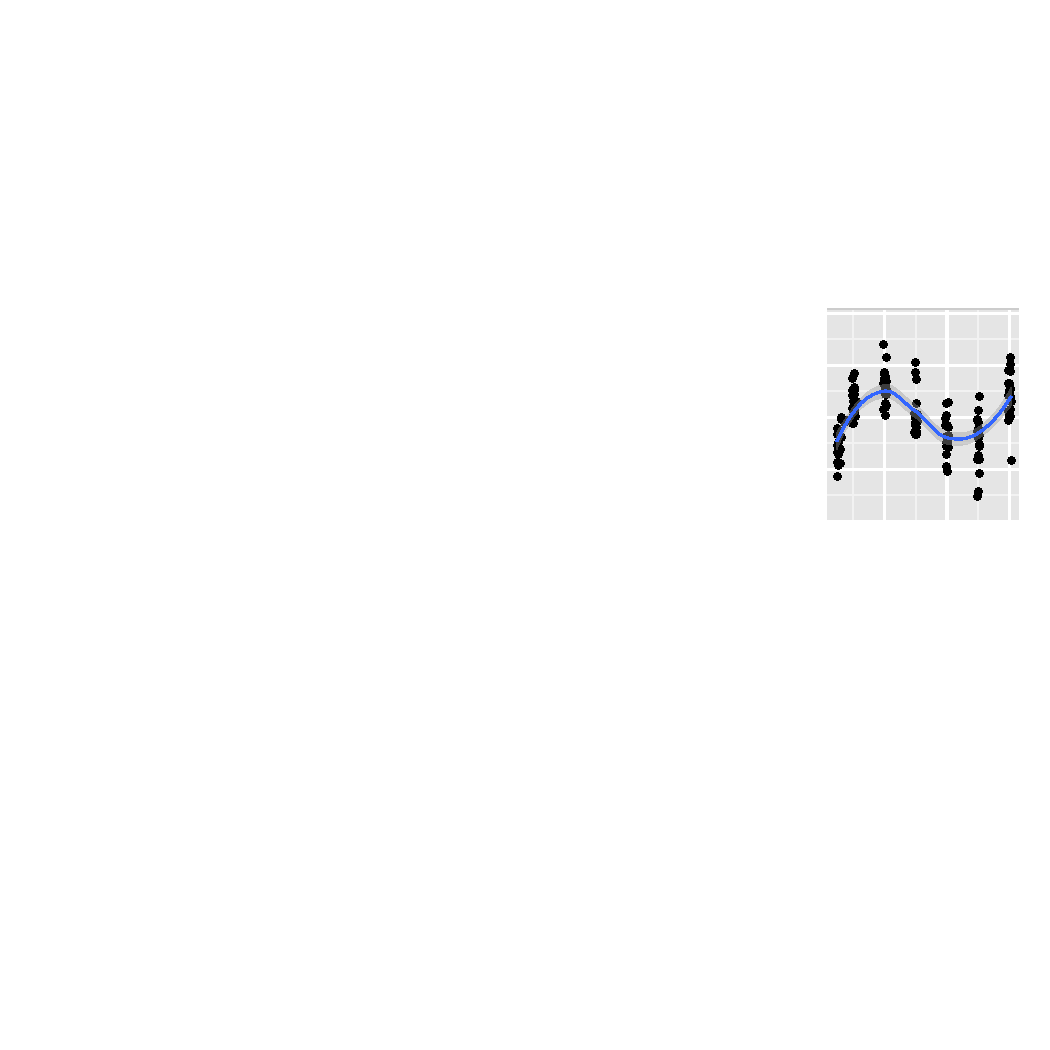
\includegraphics[width=0.05\textwidth]{dialyzernonlinear-icon}&   fig.~8& 52/55 & \hspace{-0.1in}*** & 60/62 & \hspace{-0.1in}*** & 49/52 & \hspace{-0.1in}*** & 79/83 & \hspace{-0.1in}*** & 63/67 & \hspace{-0.1in}*** & $< 10^{-4}$ \\ 
%
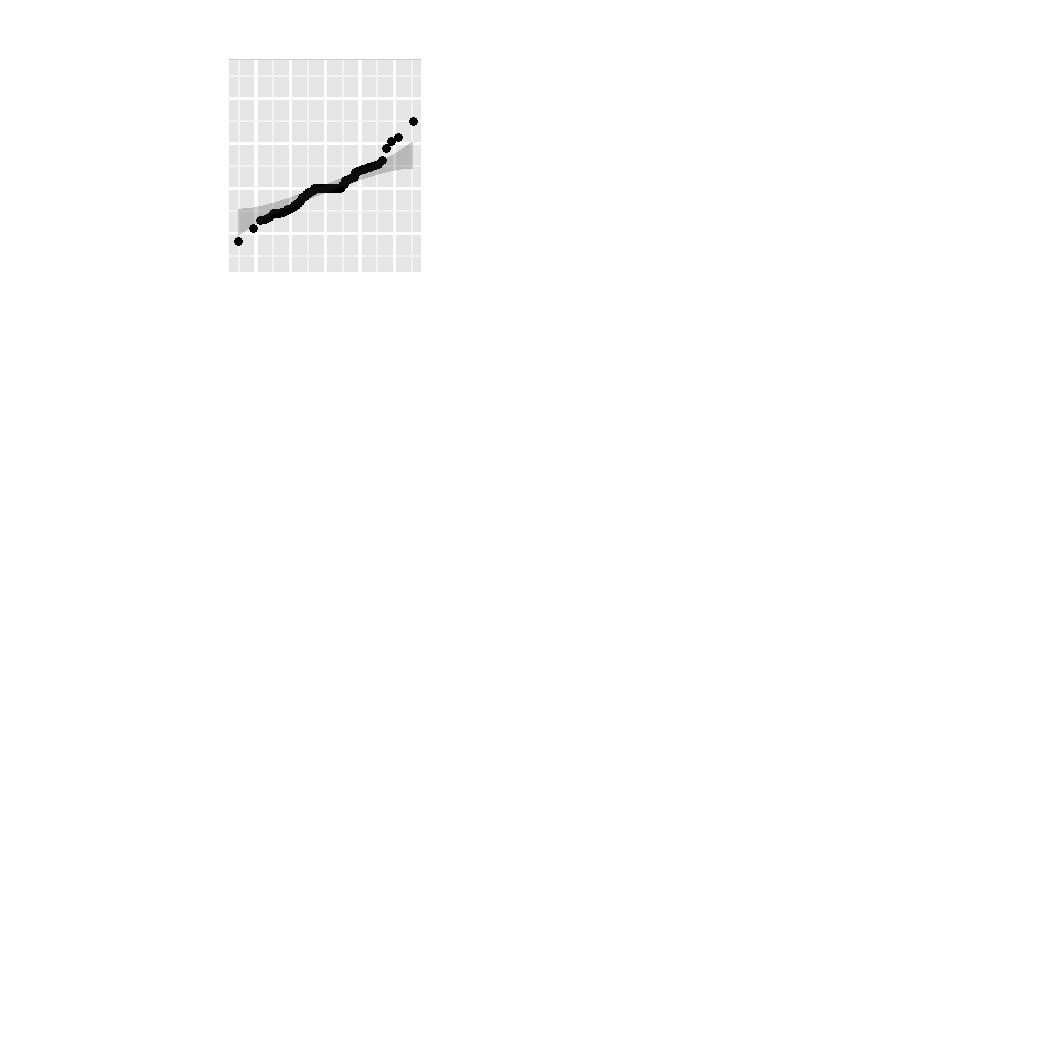
\includegraphics[width=0.05\textwidth]{radontranef-icon}&   fig.~10 & 29/70&\hspace{-0.1in}***  & 52/79&\hspace{-0.1in}*** & 0/64& & 13/59&\hspace{-0.1in}*** & 6/74& & $<10^{-5}$\\ 
\multicolumn{2}{r}{random intercept} & 0/72 & \hspace{-0.1in}  & 1/75 & \hspace{-0.1in}  & 0/68 & \hspace{-0.1in}  & 0/75 & \hspace{-0.1in}  & 2/61 & \hspace{-0.1in} & 0.8904 \\ 
\multicolumn{2}{r}{random slope} & 0/65 & \hspace{-0.1in}  & 0/64 & \hspace{-0.1in}  & 0/68 & \hspace{-0.1in}  & 0/46 & \hspace{-0.1in}  & 0/64 & \hspace{-0.1in}  & 1.0000\\ 
%
%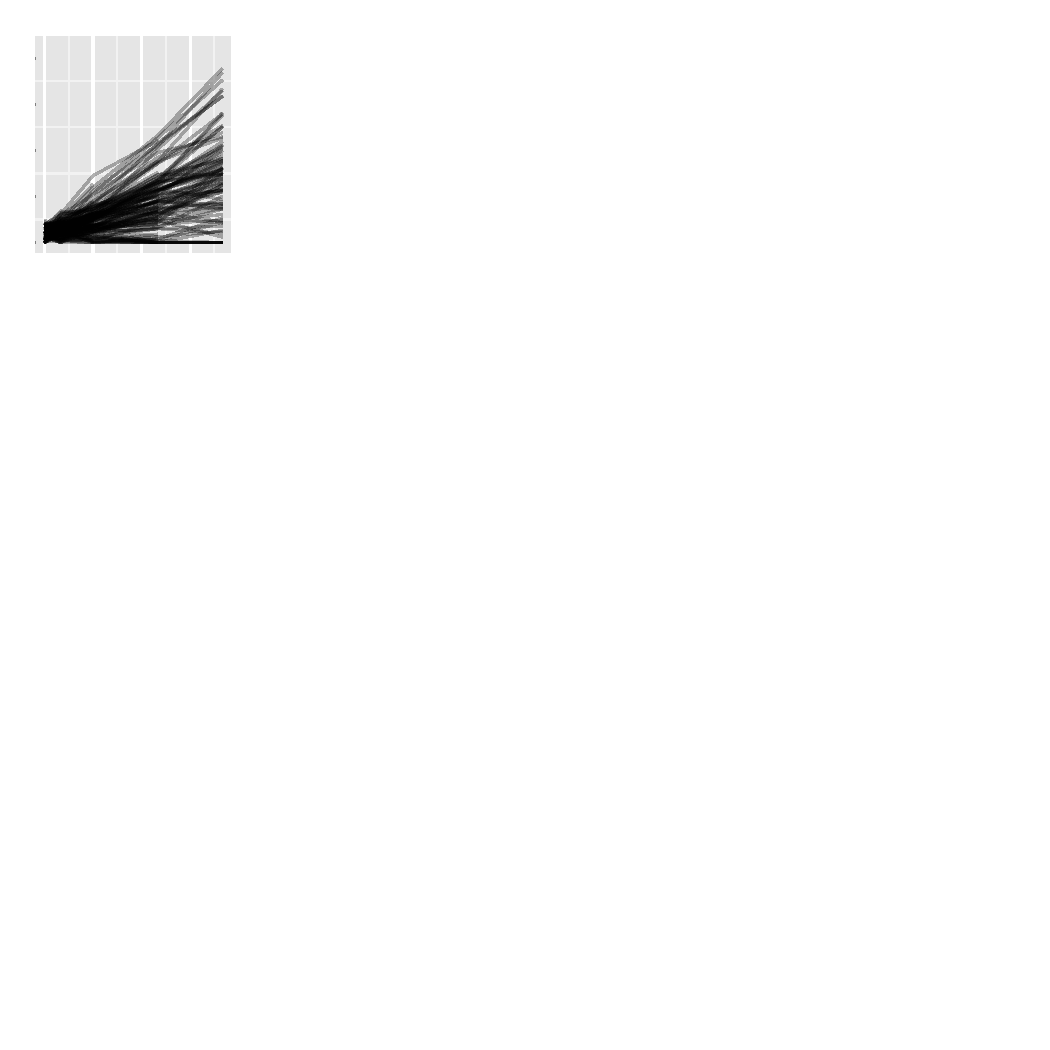
\includegraphics[width=0.05\textwidth]{autism2-fanned-icon}&   fig.~\ref{fig:autism-ranef} & 50/79&\hspace{-0.1in}***  & 26/59&\hspace{-0.1in}*** & 31/67&\hspace{-0.1in}*** & 32/72&\hspace{-0.1in}*** & 35/71&\hspace{-0.1in}*** & $<10^{-5}$\\ 
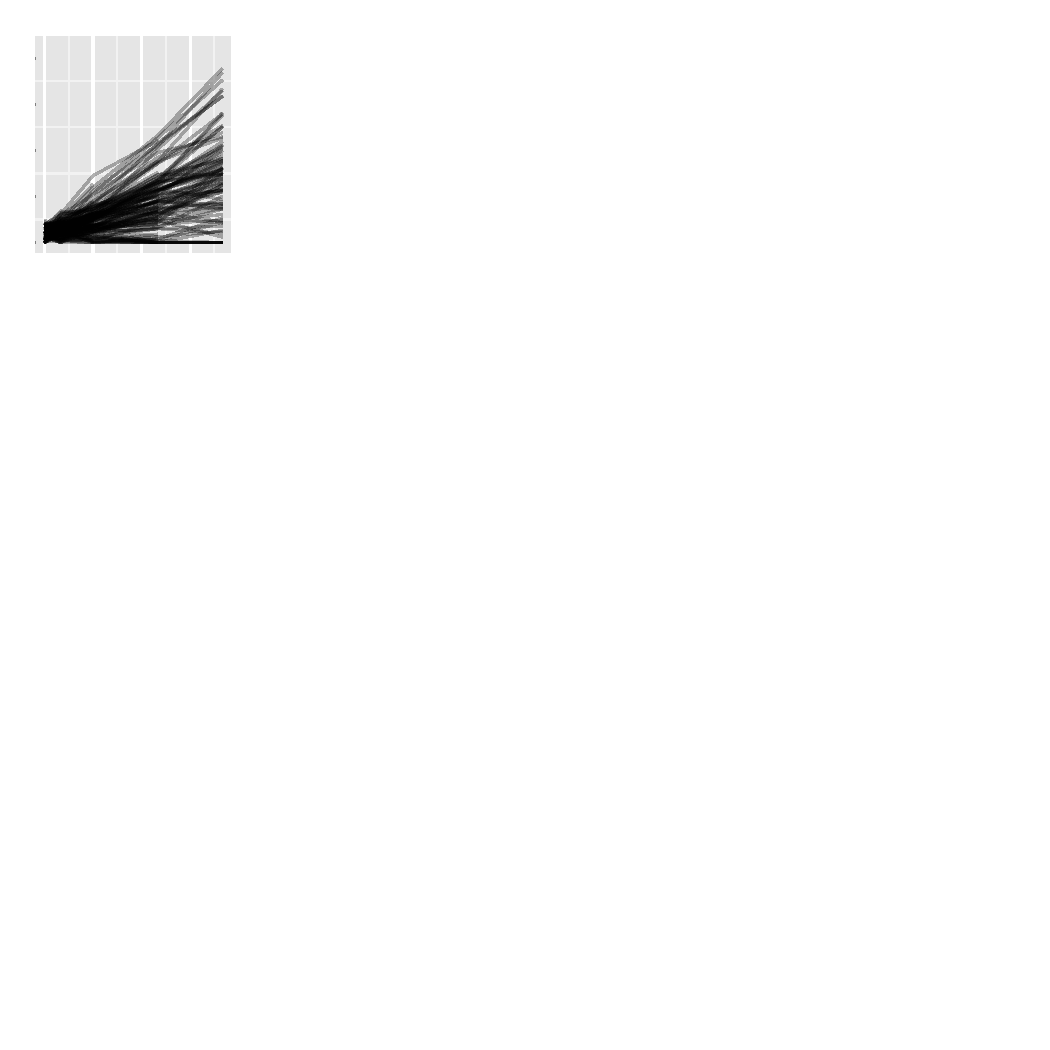
\includegraphics[width=0.05\textwidth]{autism2-fanned-icon}&   fig.~\ref{fig:autism-ranef} & 48/76 & \hspace{-0.1in}*** & 26/55 & \hspace{-0.1in}*** & 28/63 & \hspace{-0.1in}*** & 30/70 & \hspace{-0.1in}*** & 30/60 & \hspace{-0.1in}*** & $< 10^{-4}$ \\ 
%
% 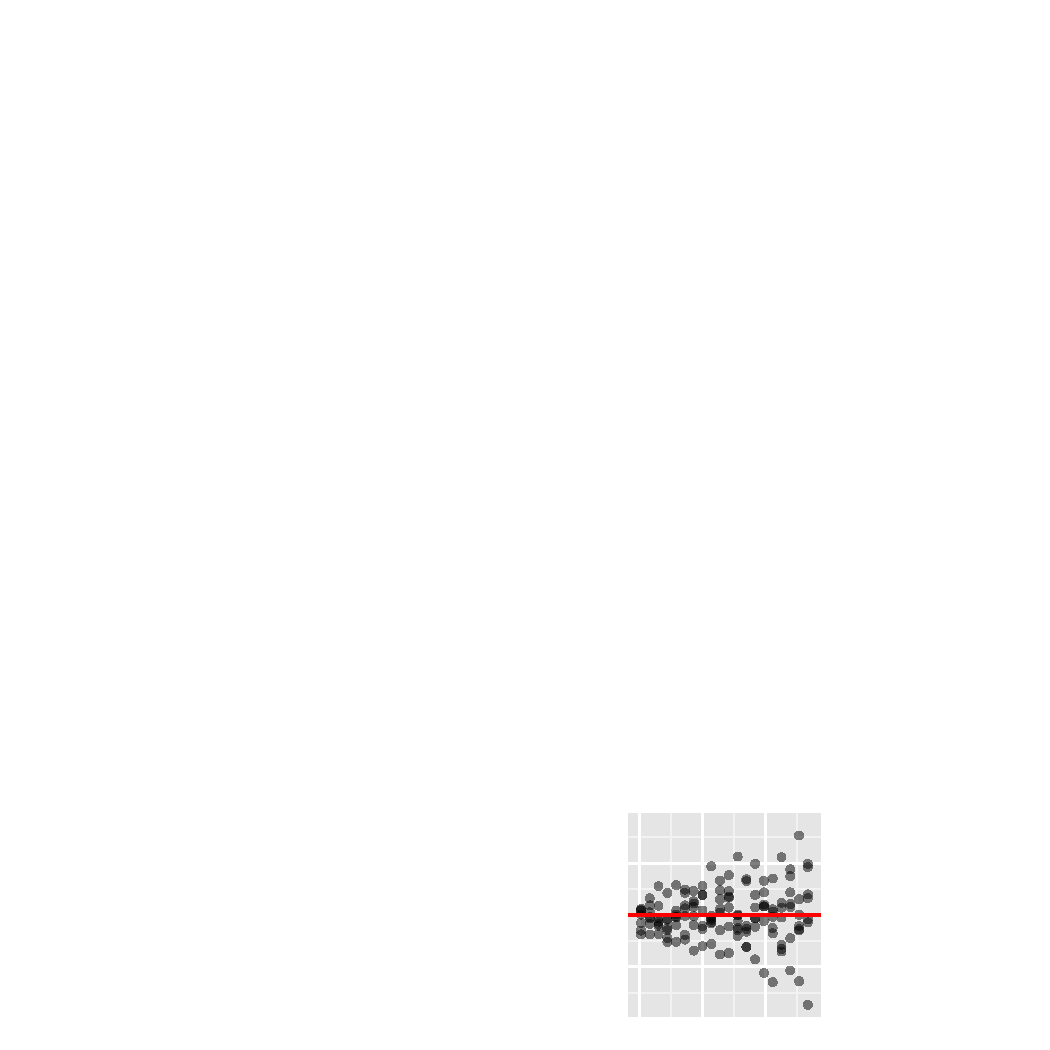
\includegraphics[width=0.05\textwidth]{homogeneous-dots-icon} & fig.~\ref{homogeneous-1}& 0/57 & \hspace{-0.1in}  & 1/71 & \hspace{-0.1in}  & 8/75 & \hspace{-0.1in}  & 0/59 & \hspace{-0.1in}  & 2/68 & \hspace{-0.1in}  & 0.7078 \\ 
 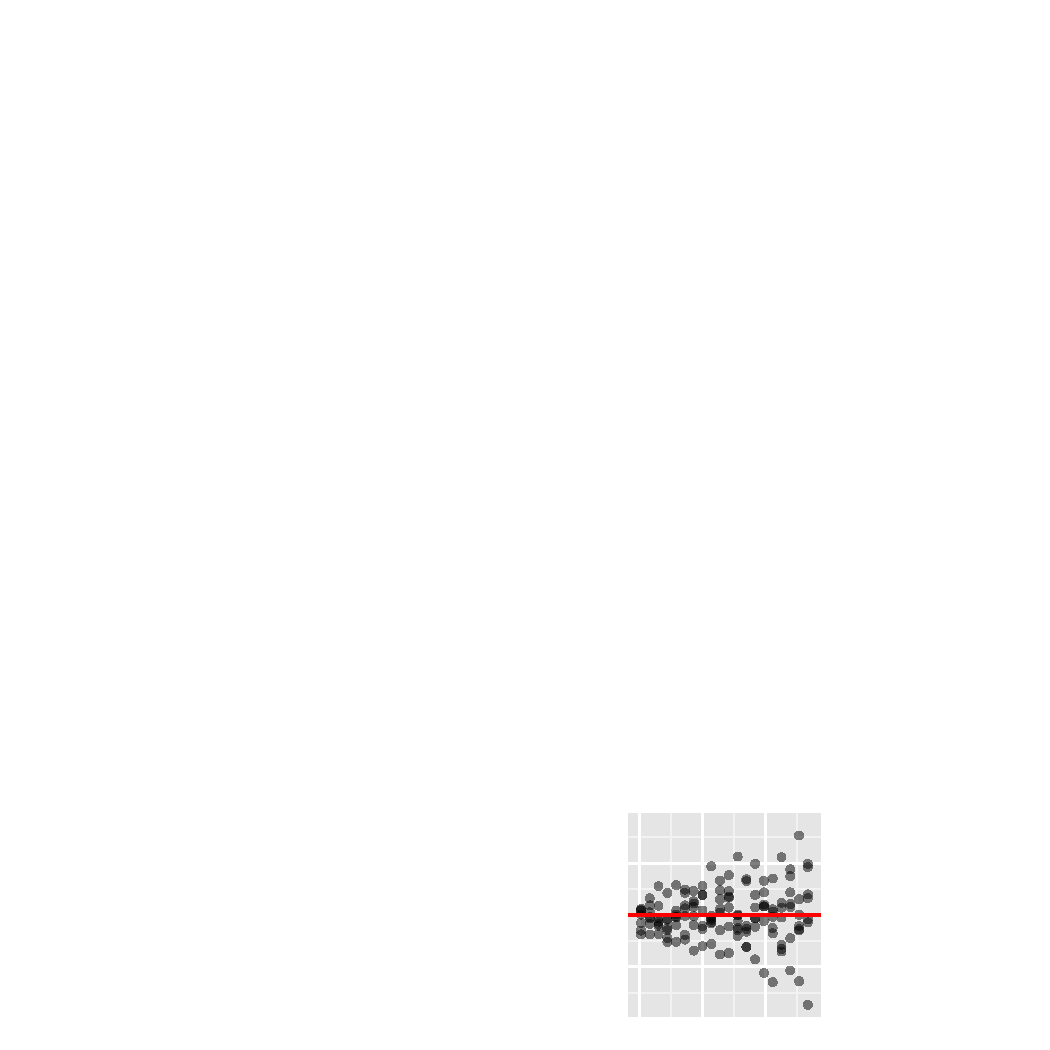
\includegraphics[width=0.05\textwidth]{homogeneous-dots-icon} & fig.~\ref{homogeneous-1}&0/57 & \hspace{-0.1in}  & 1/71 & \hspace{-0.1in}  & 8/75 & \hspace{-0.1in}  & 0/59 & \hspace{-0.1in}  & 2/68 & \hspace{-0.1in}  & 0.6448 \\ 
 
%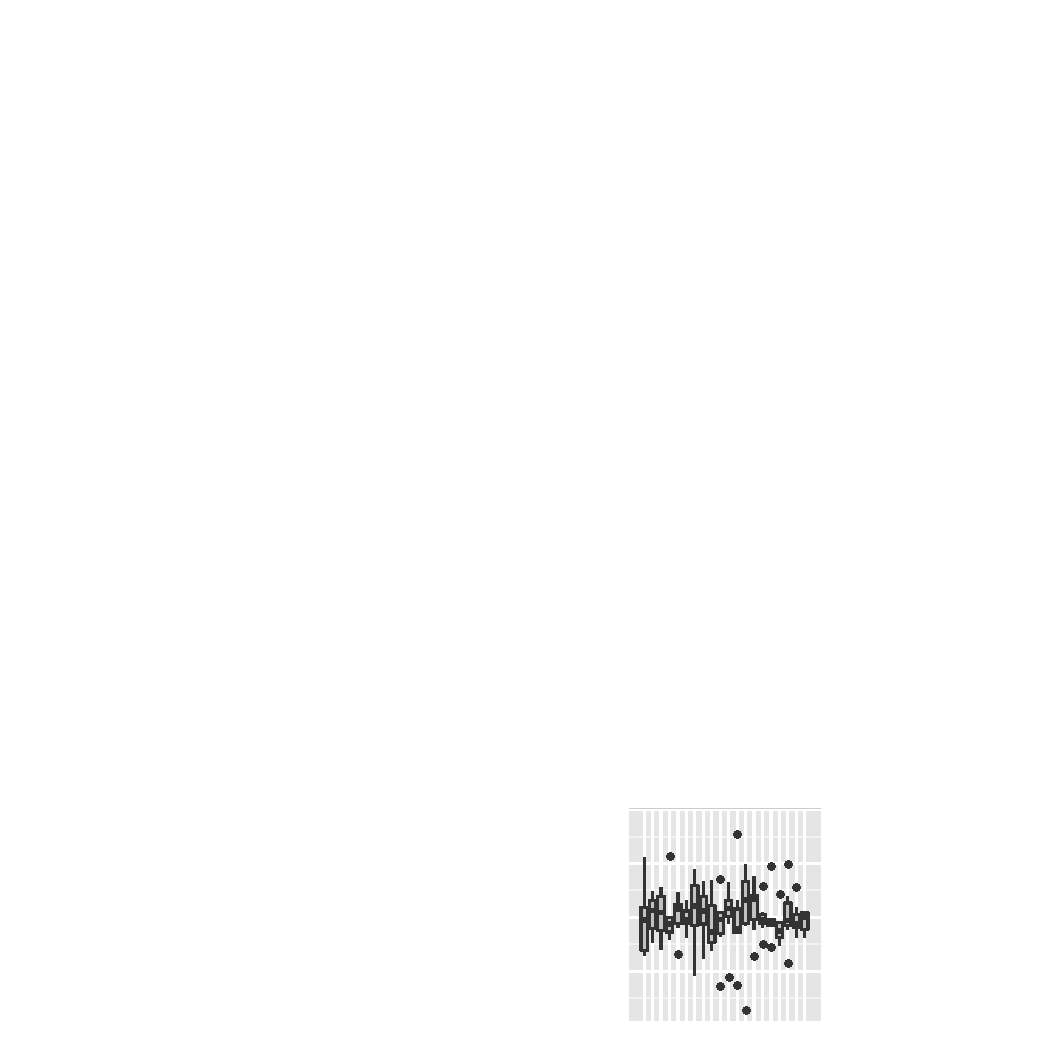
\includegraphics[width=0.05\textwidth]{homogeneous-bp-icon} &  fig.~\ref{homogeneous-2}& 23/61 & \hspace{-0.1in}*** & 38/72 & \hspace{-0.1in}*** & 29/59 & \hspace{-0.1in}*** & 22/70 & \hspace{-0.1in}*** & 35/62 & \hspace{-0.1in}*** & $<10^{-5}$\\ 
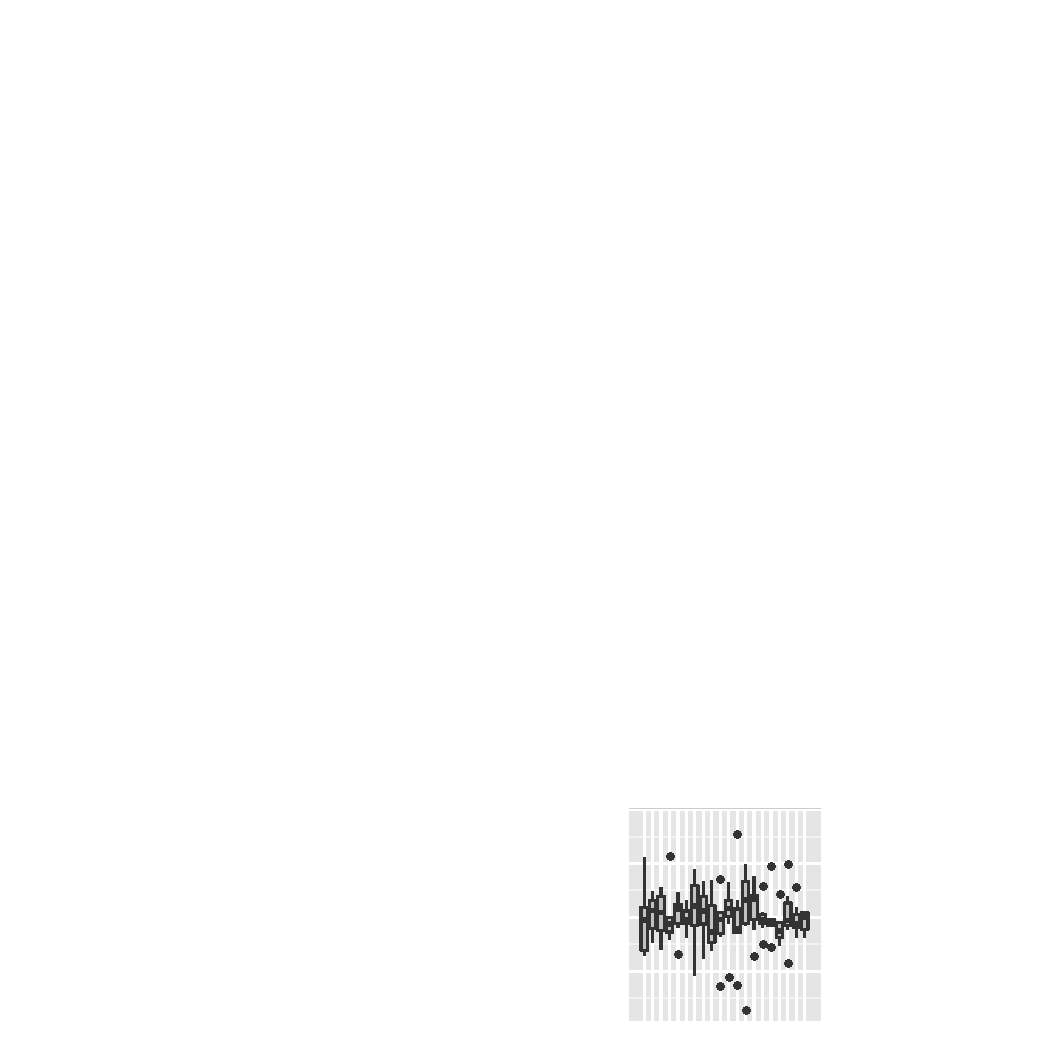
\includegraphics[width=0.05\textwidth]{homogeneous-bp-icon} &  fig.~\ref{homogeneous-2}& 26/63 & \hspace{-0.1in}*** & 48/75 & \hspace{-0.1in}*** & 0/59 & \hspace{-0.1in}  & 11/56 & \hspace{-0.1in}** & 6/69 & \hspace{-0.1in}  & $< 10^{-4}$ \\ 

   \hline
\multicolumn{12}{l}{Signif. codes:  0 $\le$ *** $\le$ 0.001 $\le$ ** $\le$ 0.01 $\le$ * $\le$ 0.05 $\le$ . $\le$ 0.1 $\le$ ' ' $\le$ 1}

\end{tabular}
\end{table}



% latex table generated in R 3.1.1 by xtable 1.7-3 package
% Fri Aug 29 22:42:40 2014
\begin{table}[ht]
\caption{\label{tab:reasons} Percent of data picks,  given the reason for the choice of plot from the lineup. }
\centering
\begin{tabular}{Mrrrrrrr}
  \hline
\multicolumn{2}{c}{Lineup} & Outlier & Spread & Trend & Asymmetry & Other \\ 
  \hline

\includegraphics[width=0.05\textwidth]{examfanned-icon} &  fig.~1  & 12.8 & 24.0 & 10.9 & 5.8 & 15.9 \\ 
 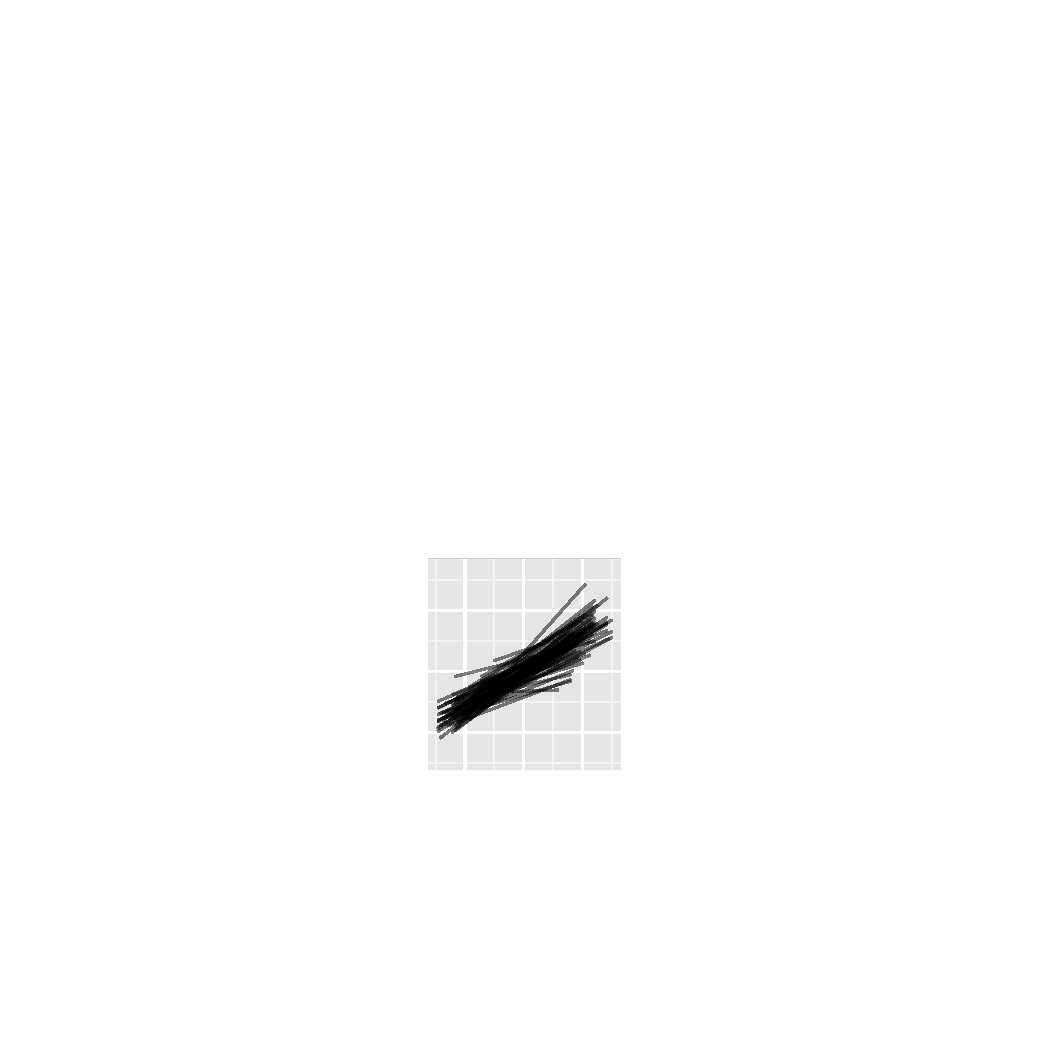
\includegraphics[width=0.05\textwidth]{exam-with-slope-icon} & fig.~3 & 2.4 & 10.6 & 3.5 & 5.4 & 0.0 \\ 

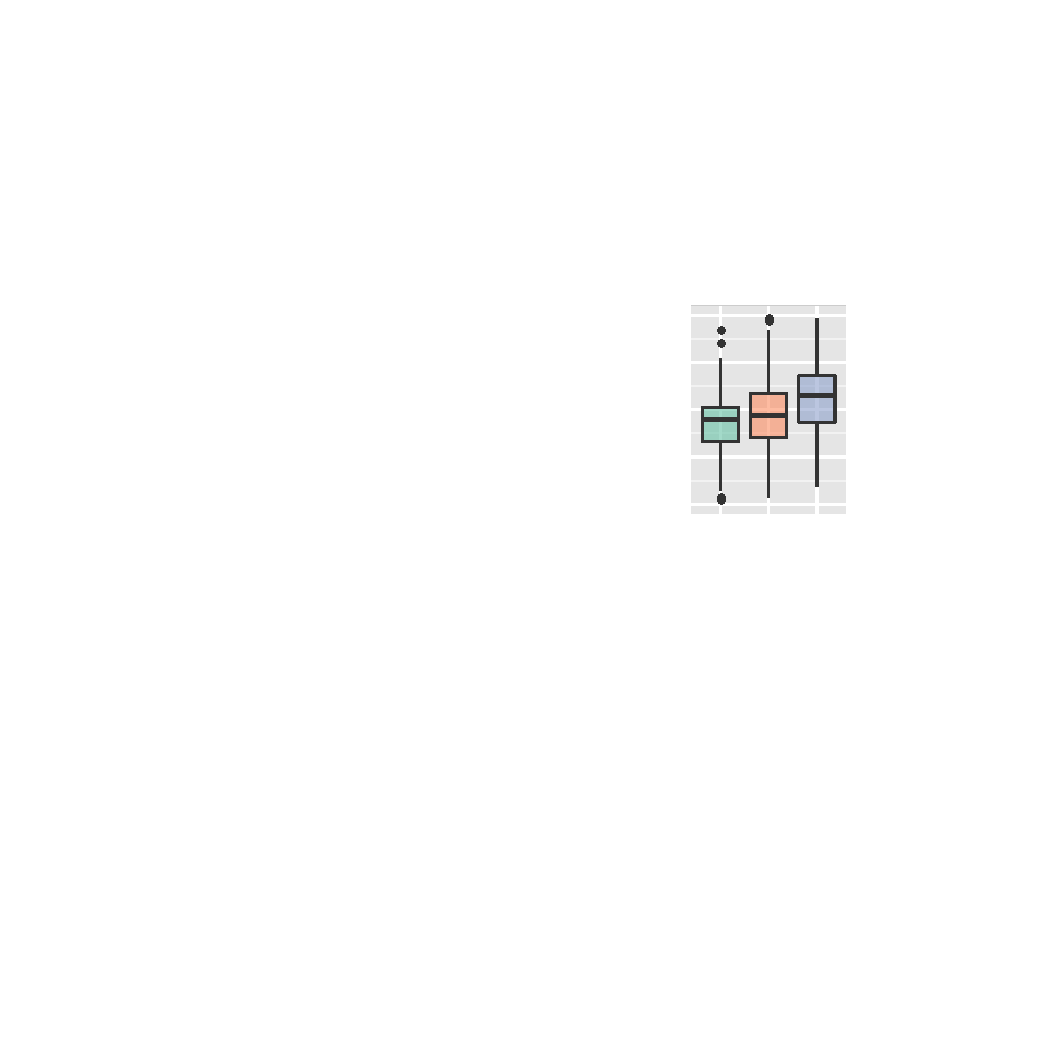
\includegraphics[width=0.05\textwidth]{autism-ordered-icon} &   fig.~2 & 73.3 & 95.5 & 92.4 & 91.0 & 80.2 \\ 
%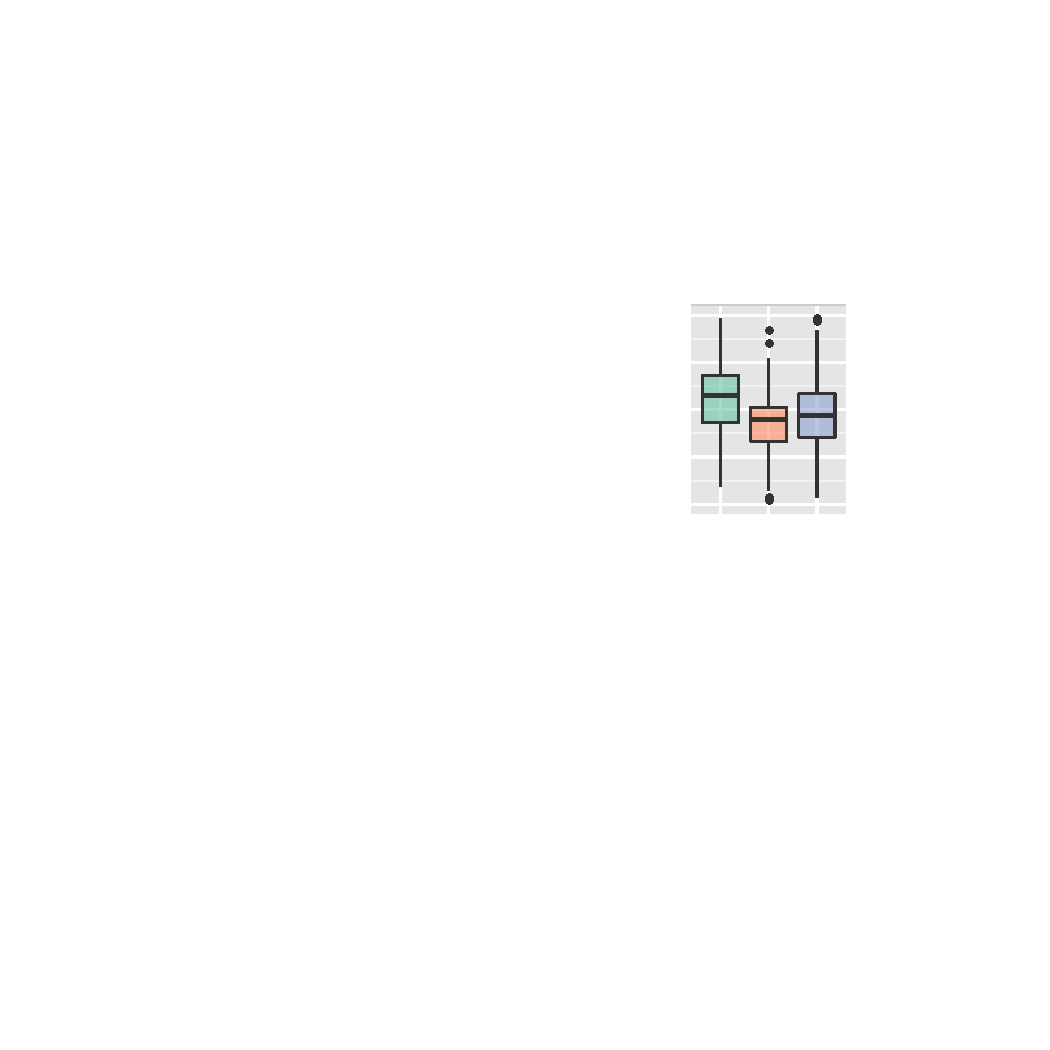
\includegraphics[width=0.05\textwidth]{autism-unordered-icon}&   fig.~\ref{fig:boxplot-unordered} & 80.2 & 99.5 & 92.4 & 91.2 & 86.2 \\ 

 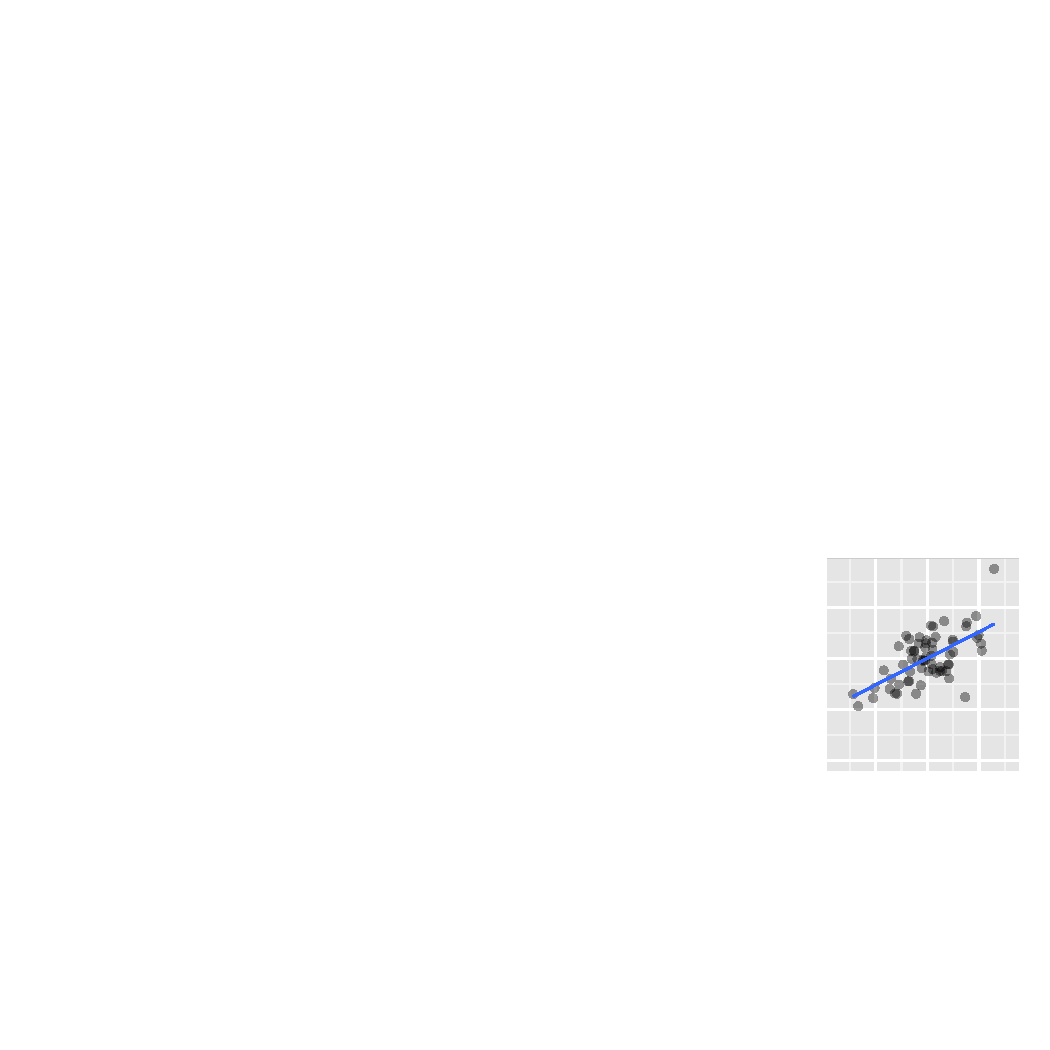
\includegraphics[width=0.05\textwidth]{examcorr-icon}&   fig.~4 & 64.5 & 34.3 & 83.4 & 70.7 & 64.9 \\ 

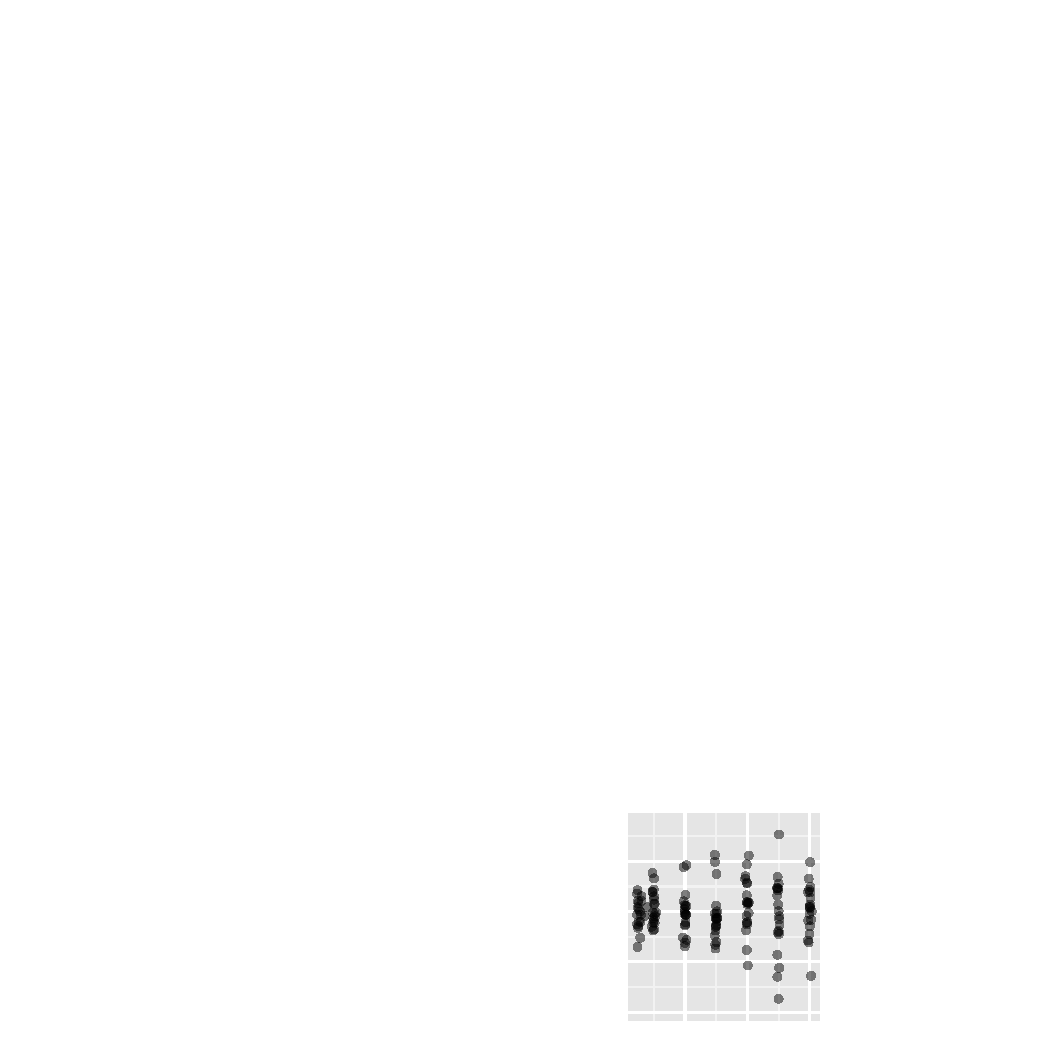
\includegraphics[width=0.05\textwidth]{dialyzerheterogeneous-icon}& fig.~5 & 19.0 & 27.3 & 29.6 & 25.8 & 19.0 \\ 
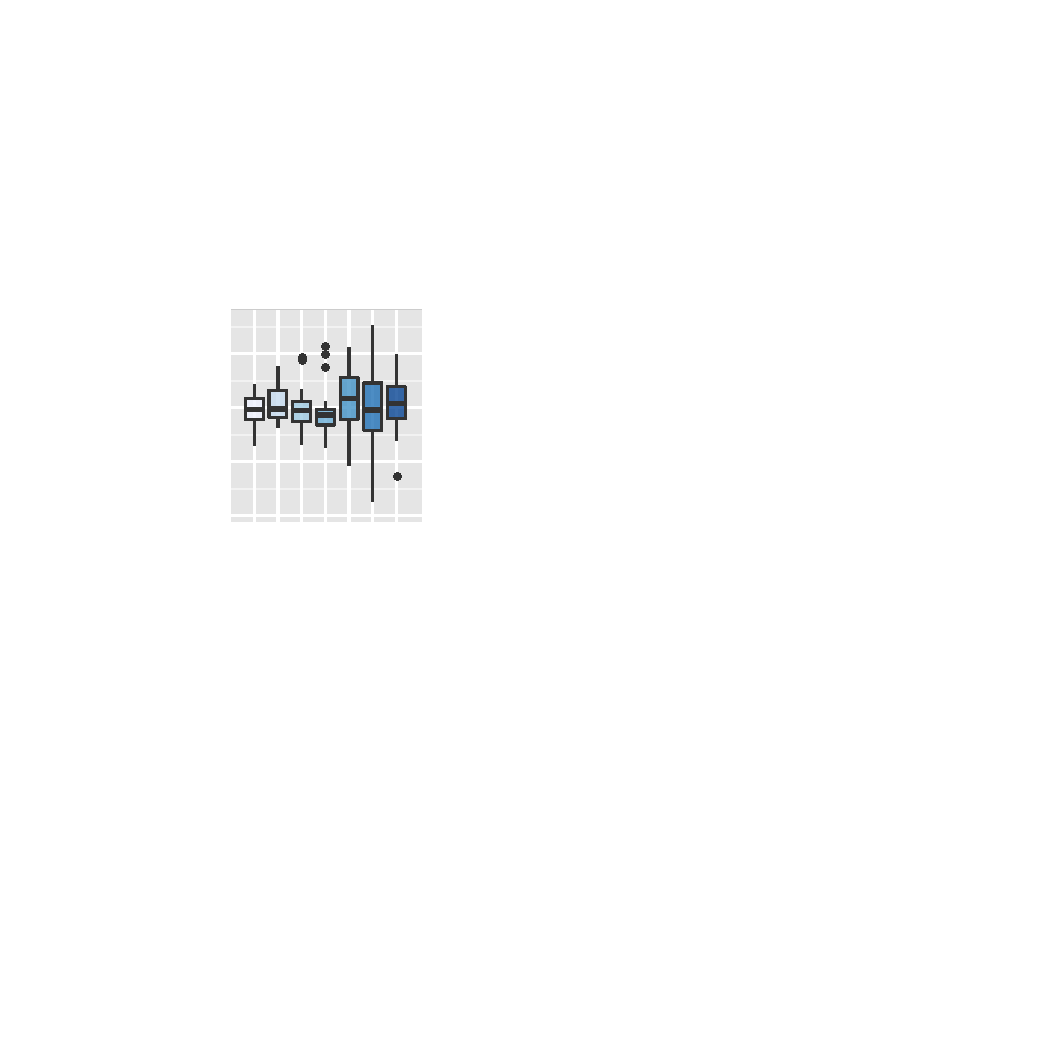
\includegraphics[width=0.05\textwidth]{dialyzerheterogeneous-bp}& fig.~\ref{fig:constvar2.bp} & 26.7 & 24.6 & 30.1 & 43.7 & 0.0 \\ 


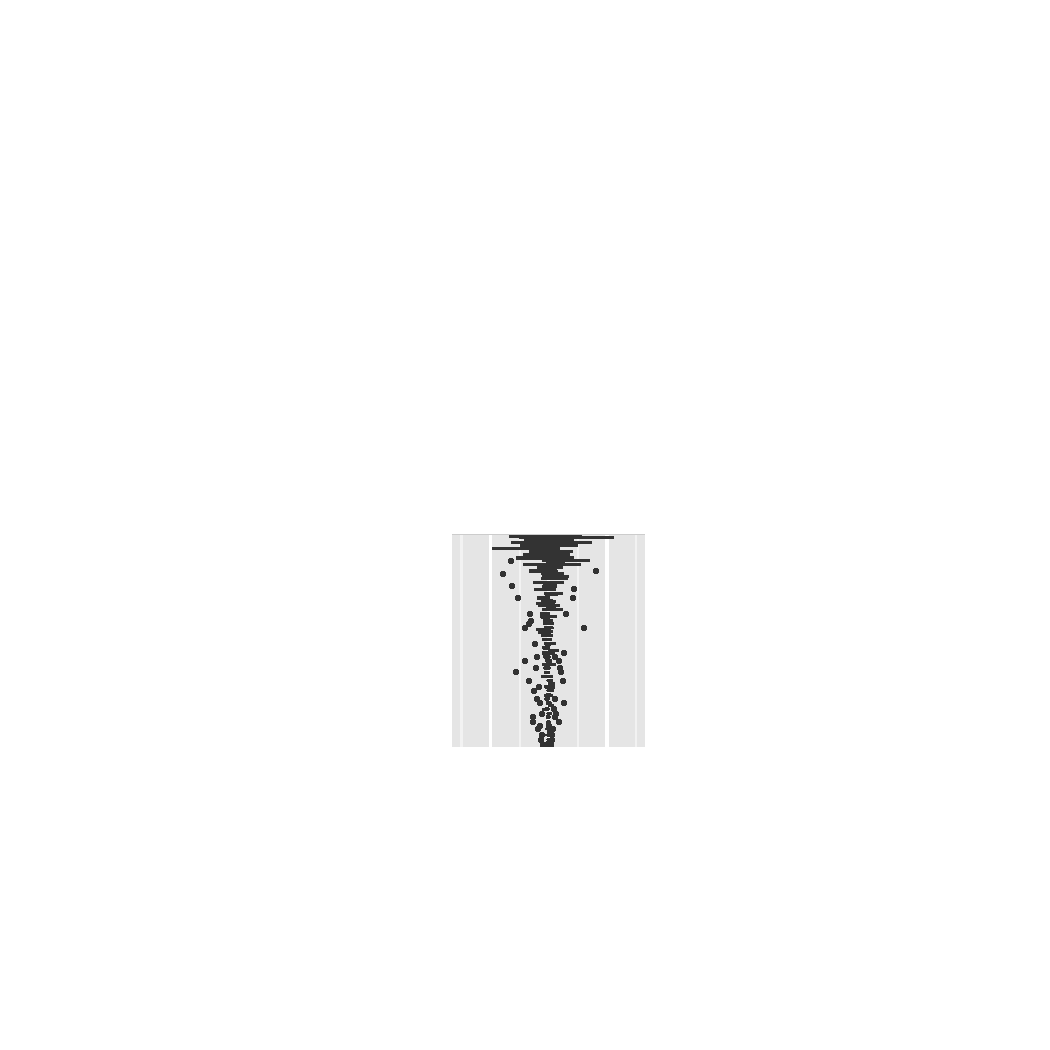
\includegraphics[width=0.05\textwidth]{cyclone-icon}&   fig.~6 & 49.6 & 49.5 & 77.7 & 79.4 & 91.8 \\ 
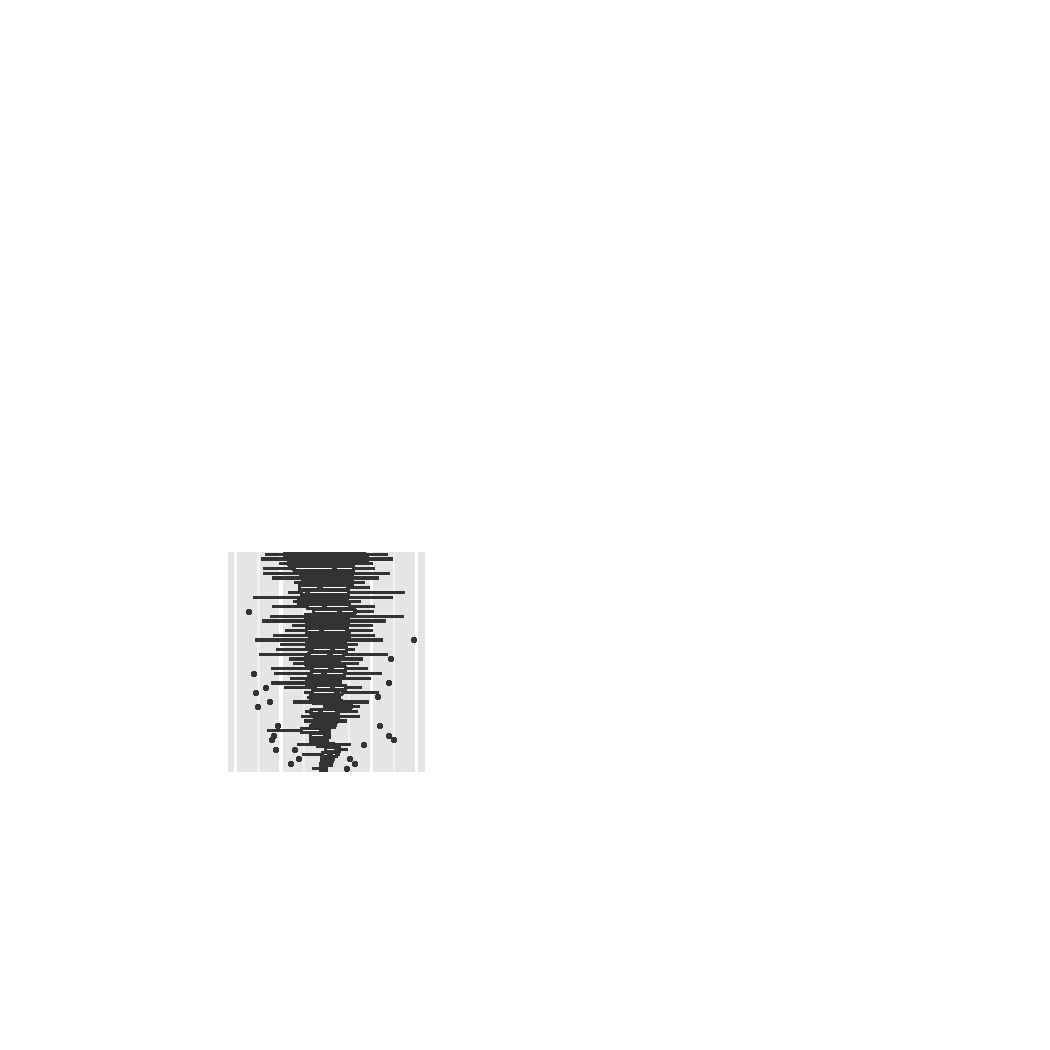
\includegraphics[width=0.05\textwidth]{cyclone-good-icon}&   fig.~7  & 4.2 & 0.6 & 2.4 & 6.8 & 0.0 \\ 

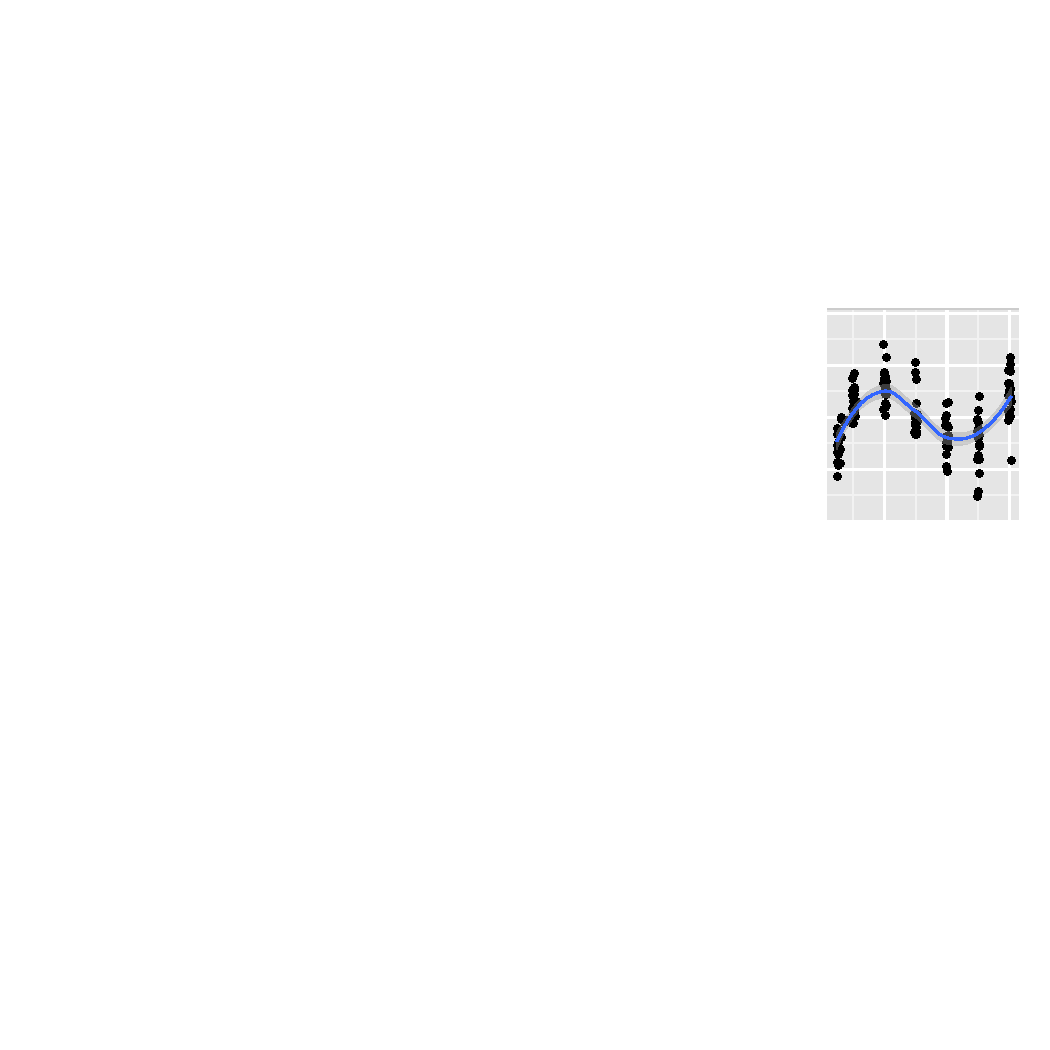
\includegraphics[width=0.05\textwidth]{dialyzernonlinear-icon}&   fig.~8 & 84.0 & 87.4 & 98.3 & 98.1 & 100.0 \\ 
%  turk11-electoral & 14.9 & 15.4 & 10.8 & 27.3 & 12.7 \\ 
%  turk11-examuncorr & 21.8 & 24.5 & 21.3 & 7.0 & 7.7 \\ 

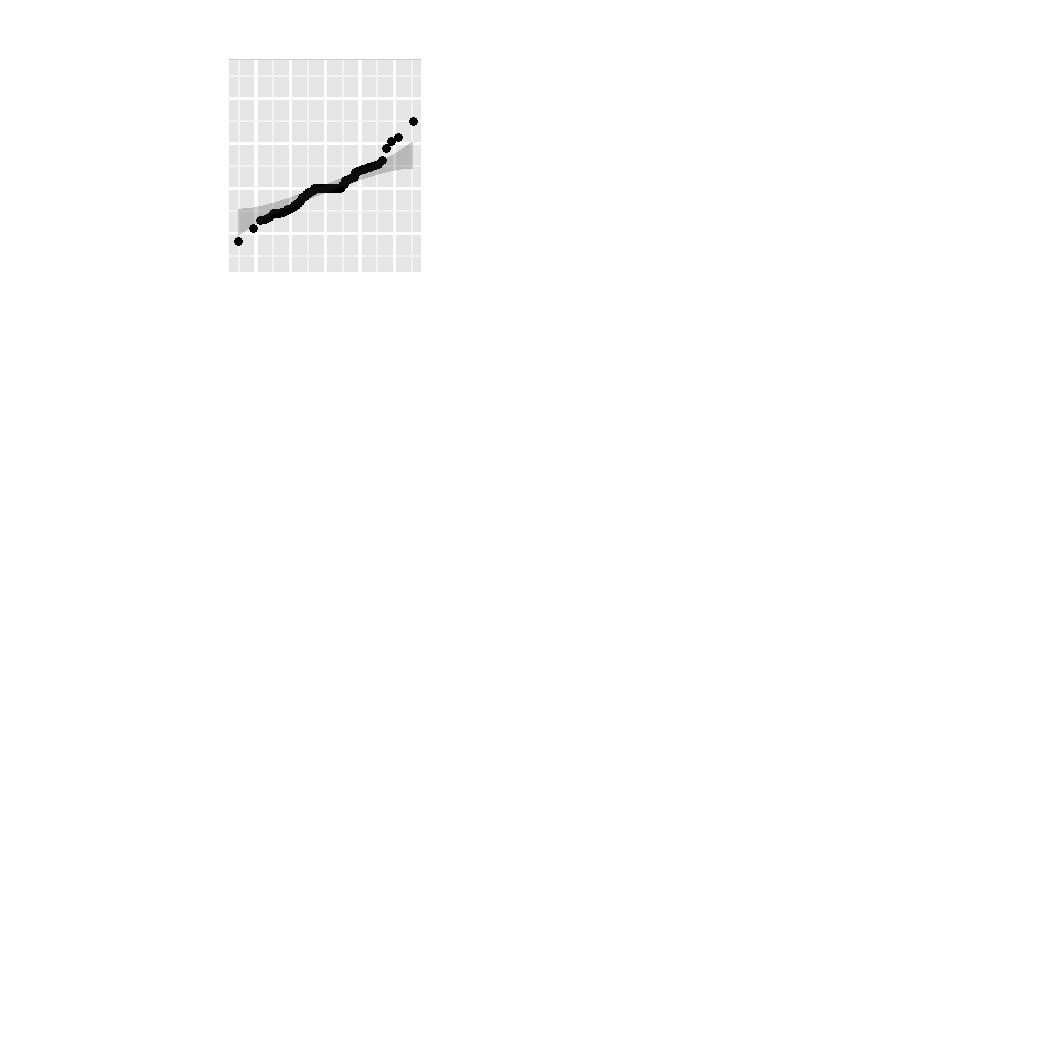
\includegraphics[width=0.05\textwidth]{radontranef-icon}&   fig.~10 & 37.8 & 49.2 & 19.6 & 4.4 & 10.9 \\ 
\multicolumn{2}{r}{random intercept} & 1.5 & 0.0 & 1.1 & 0.0 & 0.0 \\ 
\multicolumn{2}{r}{random slope} & 0.0 & 0.0 & 0.0 & 0.0 & 0.0 \\ 
 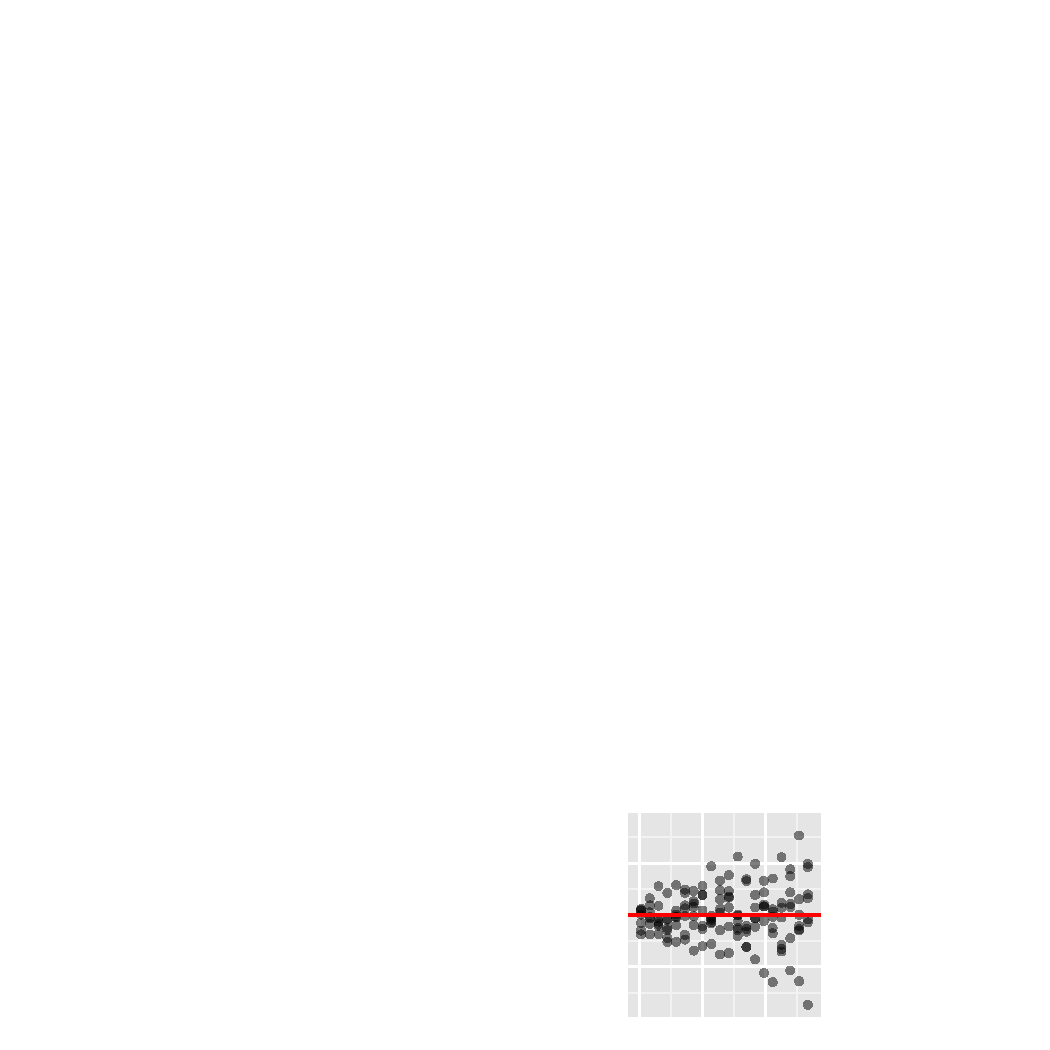
\includegraphics[width=0.05\textwidth]{homogeneous-dots-icon} & fig.~\ref{homogeneous-1} & 2.4 & 3.0 & 7.6 & 4.8 & 0.0 \\ 
 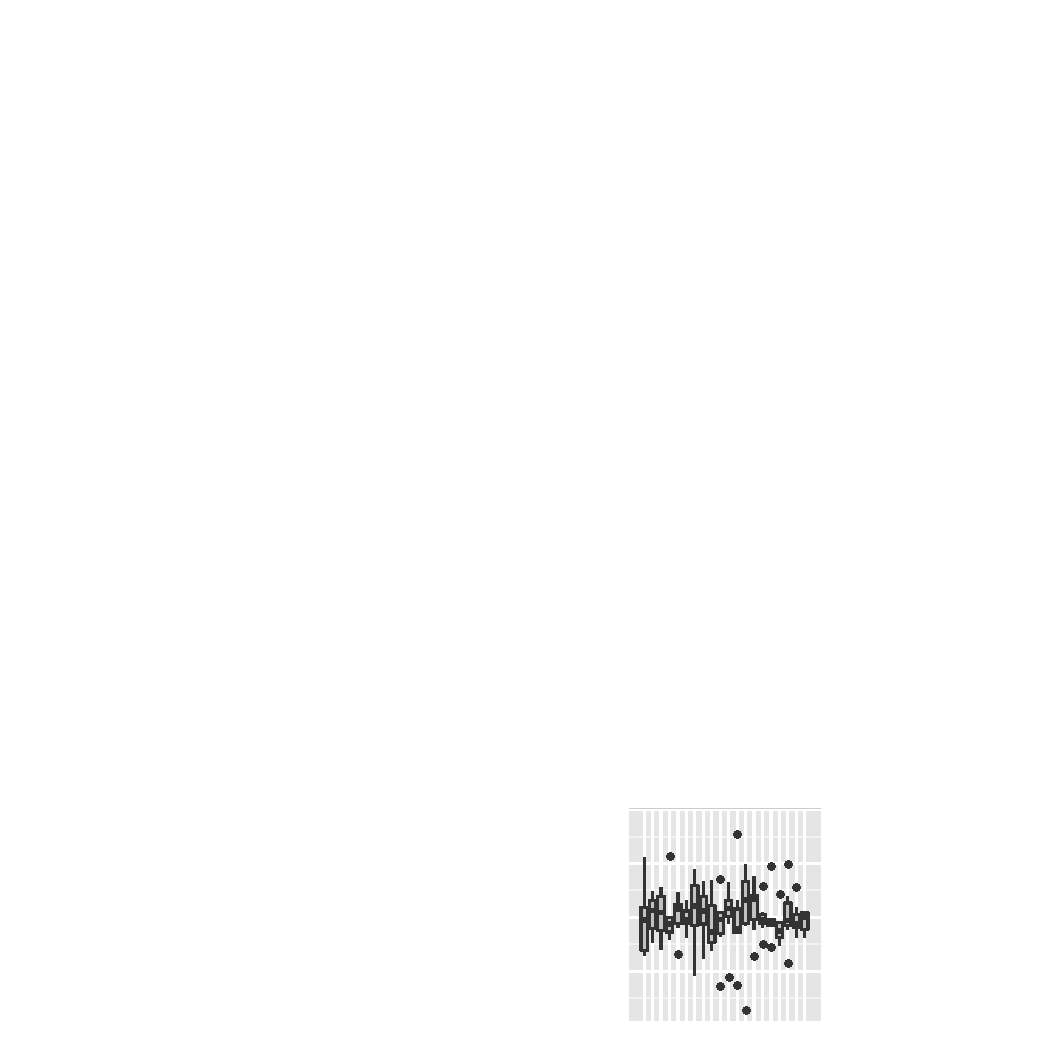
\includegraphics[width=0.05\textwidth]{homogeneous-bp-icon} & fig.~\ref{homogeneous-2} & 56.8 & 55.1 & 20.1 & 33.9 & 22.7 \\ 
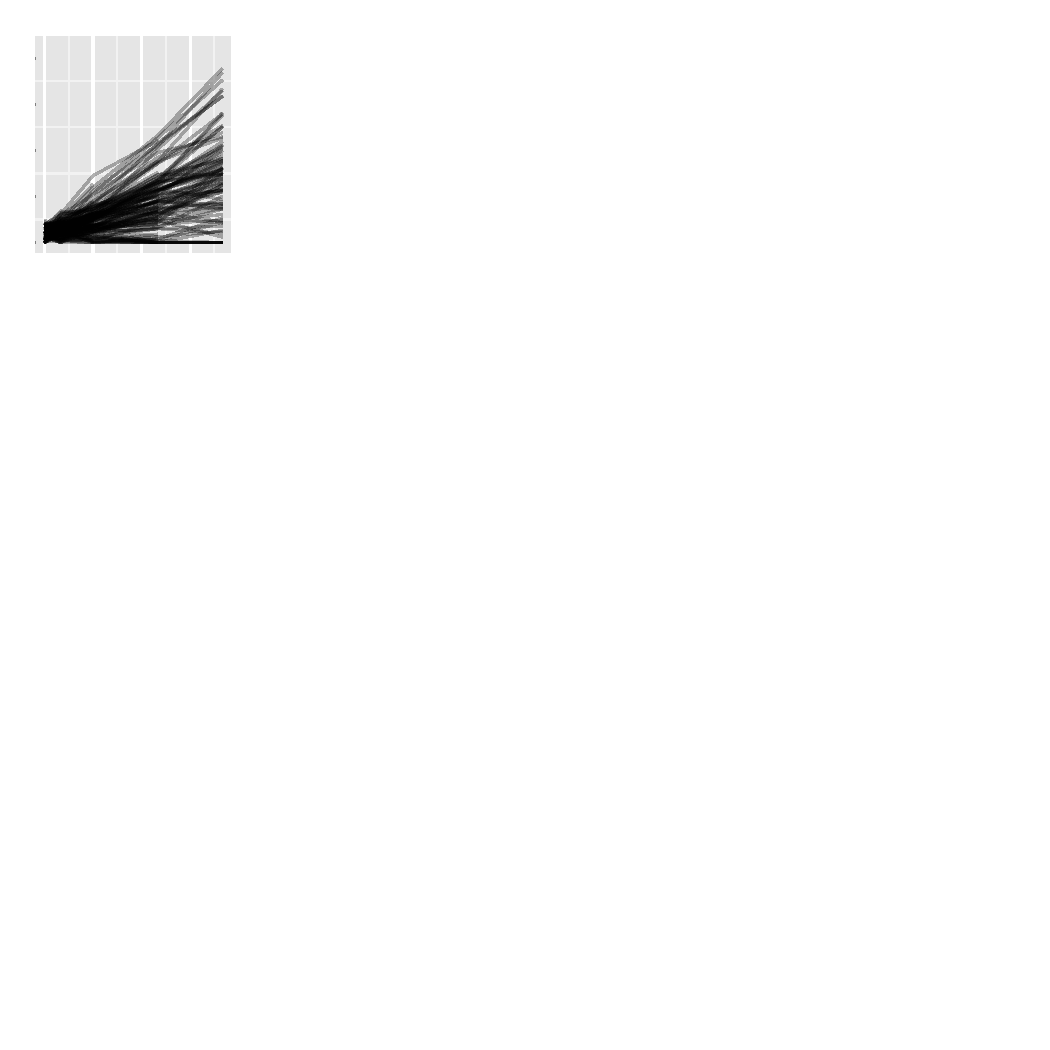
\includegraphics[width=0.05\textwidth]{autism2-fanned-icon}&   fig.~\ref{fig:autism-ranef}  & 39.2 & 33.8 & 57.9 & 78.5 & 70.0 \\ 
   \hline
\end{tabular}
\end{table}
\clearpage
%------------------------------------------------------------------------------------
\subsection{Generating null plots}\label{app:nullplots}
%------------------------------------------------------------------------------------

All of the lineups presented in this paper use a parametric bootstrap to generate plots consistent with the null hypothesis. This section outlines the parametric bootstrap for LME models and provides more detail about how the null plots were generated.

For a fitted continuous response LME model (as outlined by Equations \eqref{eq:hlm}--\eqref{eq:conditionalmod} and the intermediate discussion) the parametric bootstrap proceeds as follows:

\begin{enumerate}
\item Generate a vector of $q$ random effects (i.e., level-2 residuals) from $\mathcal{N}(\bm{0},\ \widehat{\bm{D}})$ for each group; that is, generate $\bm{b}^*_i \sim \mathcal{N}(\bm{0},\ \widehat{\bm{D}})$ for $i = 1,\ldots, g$. 
\item Generate a vector of residuals of length $n_i$ (i.e., level-1 residuals) from $\mathcal{N}(\bm{0},\ \widehat{\sigma}^2 \widehat{\bm{R}_i})$ for each group; that is, generate $\bm{\varepsilon}^*_i \sim \mathcal{N}(\bm{0},\ \widehat{\sigma}^2 \widehat{\bm{R}_i})$ for $i = 1,\ldots, g$.
\item Generate a bootstrap sample $\bm{y}_i^*$ for each group $i=1,\ldots,g$ from $\bm{y}_i^* = \bm{X}_i \widehat{\bm{\beta}} + \bm{Z}_i \bm{b}_i^* + \bm{\varepsilon}^*_i$.
\item Refit the model to the bootstrap samples.
\item Repeat steps 1--4 $B$ times.
\end{enumerate}

%We detail the models suggested in the paper for use in model selection and model checking below. 
The parametric bootstrap was used to generate the null plots in each situation. 
During model selection the simpler models are used to generate the null plots using the parametric bootstrap, while model checking bootstraps the original model to generate null plots.

\paragraph{Selecting fixed effects.} To use lineup tests to determine whether a variable should be included in the fitted model we must generate null plots from a model \emph{excluding} the variable in question. Let $\bm{X}_i^{(c)}$ denote the design matrix for the fixed effects with the $c$th column  deleted. We use the model 
%
\[
\bm{y}_i = \bm{X}_i^{(c)} \bm{\beta} + \bm{Z}_i \bm{b}_i + \bm{\varepsilon}_i
\]
%
to generate the null plots.

\paragraph{Selecting random effects structure.} To use a lineup test to determine whether a random effect should be included in the fitted model we must generate null plots from a model \emph{excluding} the random effect in question. This results in a model of the form of~\eqref{eq:hlm} with the column of $\bm{Z}_i$ corresponding to the random effect in question deleted, and a random effects vector $\bm{b}_i$ of length $q-1$. To determine whether it is necessary to allow the random effects to be correlated, the null plots are generated using a model where the covariance matrix of the random effects $\bm{D}$ has zero entries in the appropriate off diagonal entries.

\paragraph{Model checking.} Generating the null plots used for model checking is a direct application of the parametric bootstrap as detailed above to obtain $B$ fitted models from which the appropriate aspects are extracted.



%------------------------------------------------------------------------------------
\subsection{Additional lineups included in the study}\label{app:morelineups}
%------------------------------------------------------------------------------------

This section includes two lineups that were included in the  MTurk study, but were not discussed in the paper. 

Figure~\ref{fig:constvar2.bp} contains a box plot representation of the same data as Figure~5 in the paper, but categorizes pressure into seven categories, and shows residuals in the form of box plots. In order to preserve the appearance of continuity on the $x$-axis we used a color scheme to fill the boxes with deepening shades of blue from left to right. In this form 23 out of 70 observers identify the plot of the data.  This is consistent with the other design.

\begin{figure}[hbt]
	\centering
	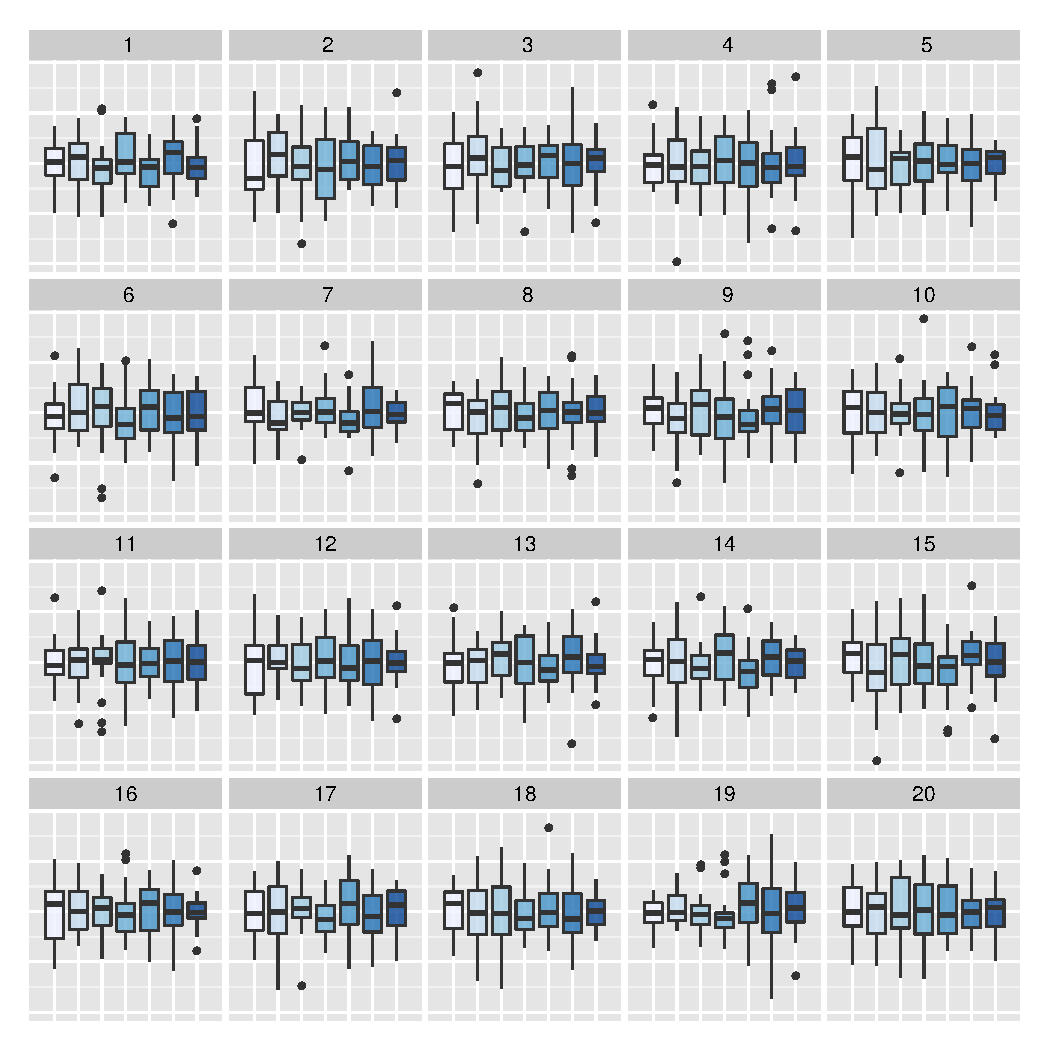
\includegraphics[width=0.8\textwidth]{dialyzerheterogeneous-bp-19.pdf}
	\caption{\label{fig:constvar2.bp} 
	Alternative box plot  Lineup testing homogeneity of the level-1 residuals. Which of the plots is the most different? Which feature led you to your choice?}
%	Lineup of 20 scatterplots of level-1 residuals against pressure used to test the assumption of homogeneous level-1 residual variance for the dialyzer study.  Which is the real plot?}
\end{figure}


%%%%%%%%%%%%%%%%%%%




%\hhnote{reference to corresponding lineup in main paper}
Figure~\ref{fig:autism-ranef} displays another lineup testing the adequacy of the random effects specification  (see Section~3.2 of the paper) using data from the autism study. The null plots were generated from a model containing only a linear random slope, so if the true plot in panel \#($\sqrt{16} + 12$) is identified it provides support for the inadequacy of this specification, and the need for additional random effects. %Figure~\ref{fig:boxplot-unordered} shows similar data  as Figure~\ref{fig:boxplot-ordered}, where categories were re-labelled to investigate whether the order might have an effect on people's choices. Interestingly, the power is the same, and observers still identify 'trend' as one of the top reason for their choice.

\begin{figure}
	\centering
	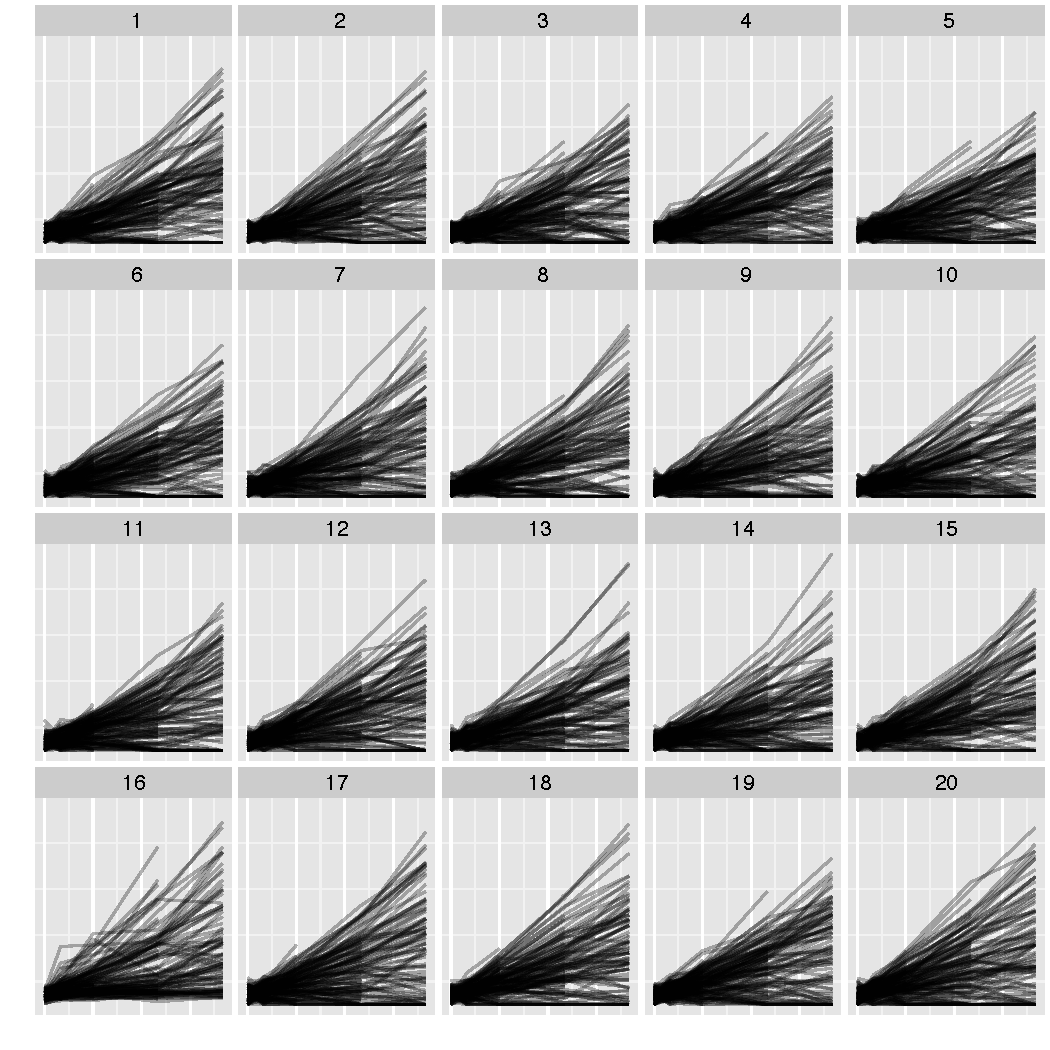
\includegraphics[width=0.8\textwidth]{autism-fanned2-16.pdf}
	\caption{\label{fig:autism-ranef} Which of the plots is the most different? Which feature led you to your choice? }
\end{figure}

%\begin{figure}[h]
%	\centering
%	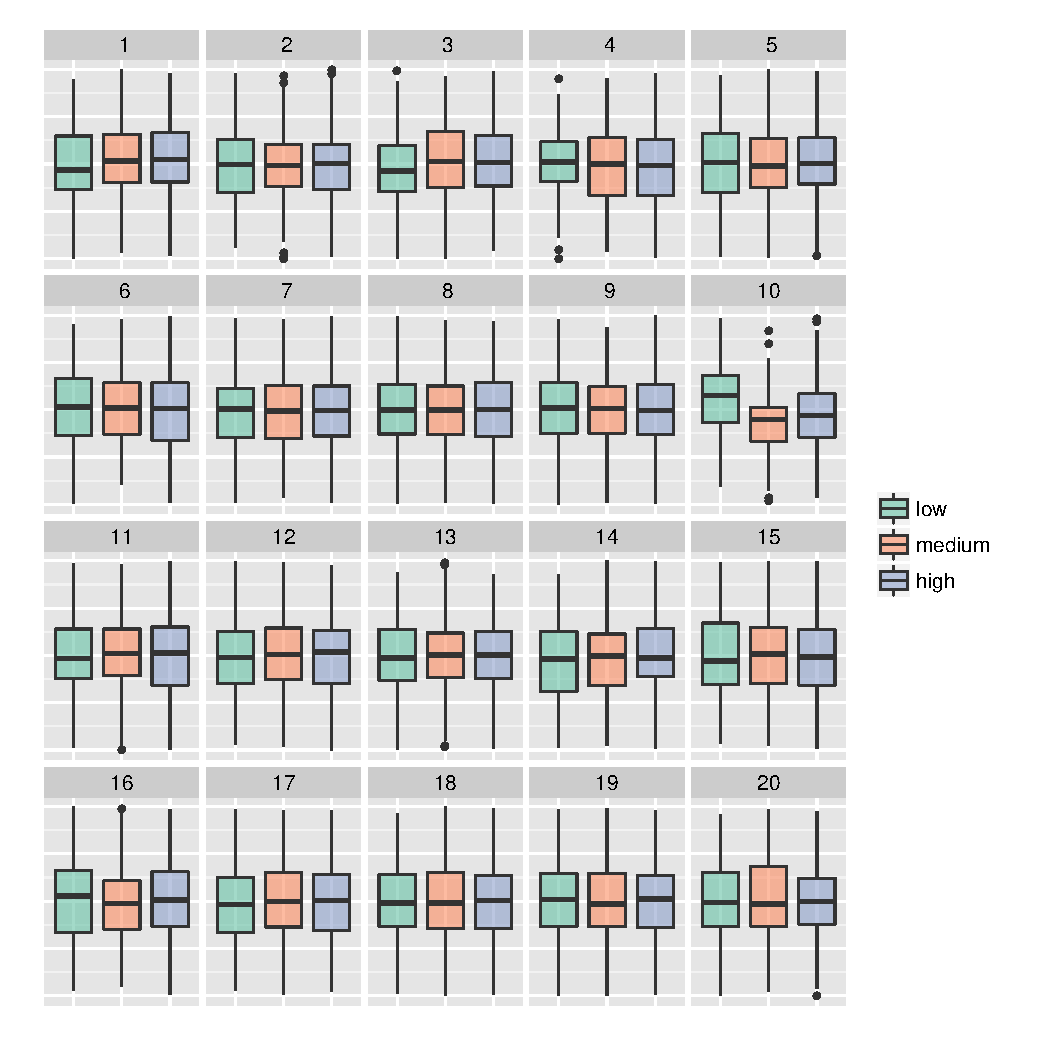
\includegraphics[width=0.8\textwidth]{autism2-unordered-10.pdf}
%	\caption{\label{fig:boxplot-unordered} An alternative layout of Figure~\ref{fig:boxplot-ordered}, where the boxplots are ordered as they are for inference. Which of the plots is the most different? Which feature led you to your choice?}
%\end{figure}

%%%%%%%%%%%%%%%%%%%


\begin{figure}[hbt]
	\centering
	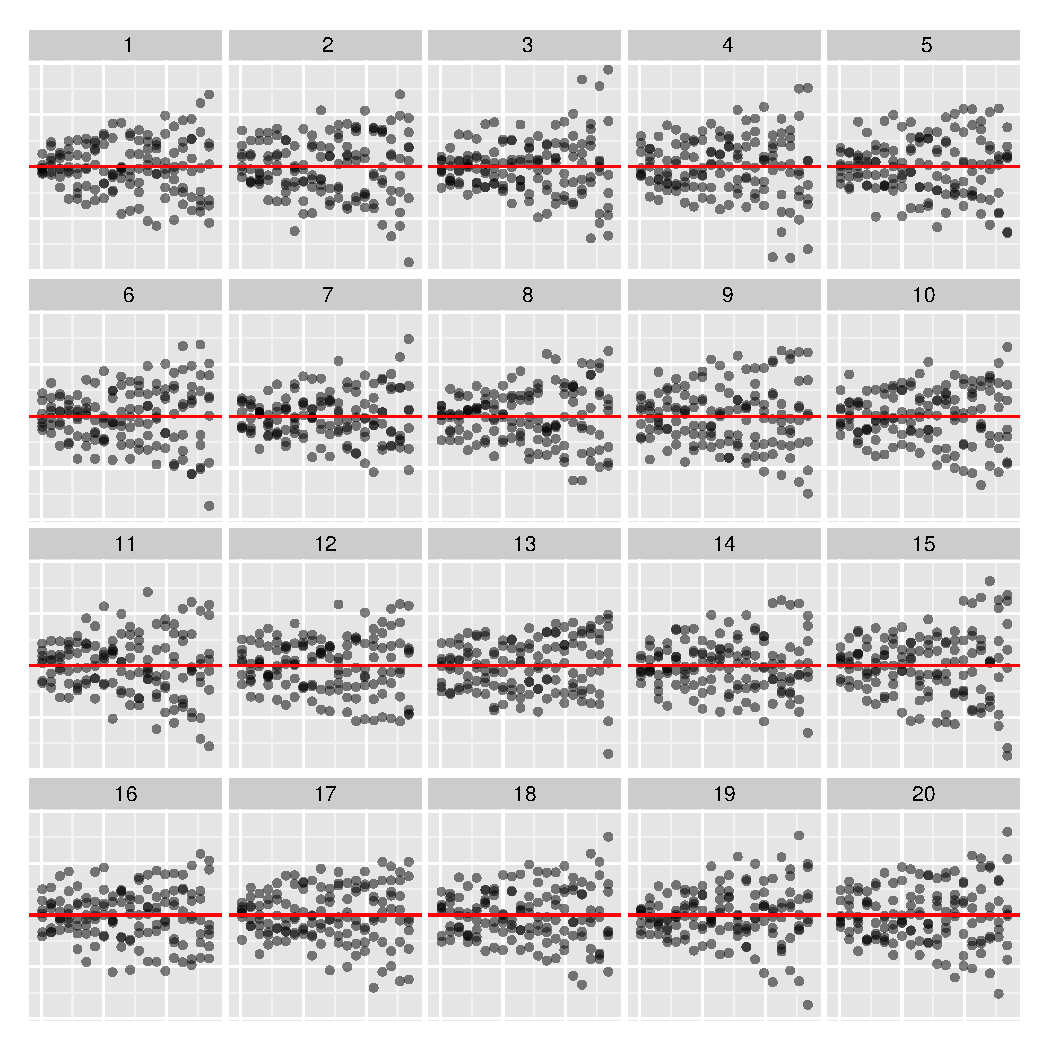
\includegraphics[width=0.8\textwidth]{dialyzerhomogeneous-dots-1-19.pdf}
	\caption{\label{homogeneous-1}
	Lineup testing homogeneity of the level-1 residuals. Which of the plots is the most different? Which feature led you to your choice?}
%	Lineup of 20 scatterplots of level-1 residuals against pressure used to test the assumption of homogeneous level-1 residual variance for the dialyzer study.  Which is the real plot?}
\end{figure}
\begin{figure}[hbt]
	\centering
	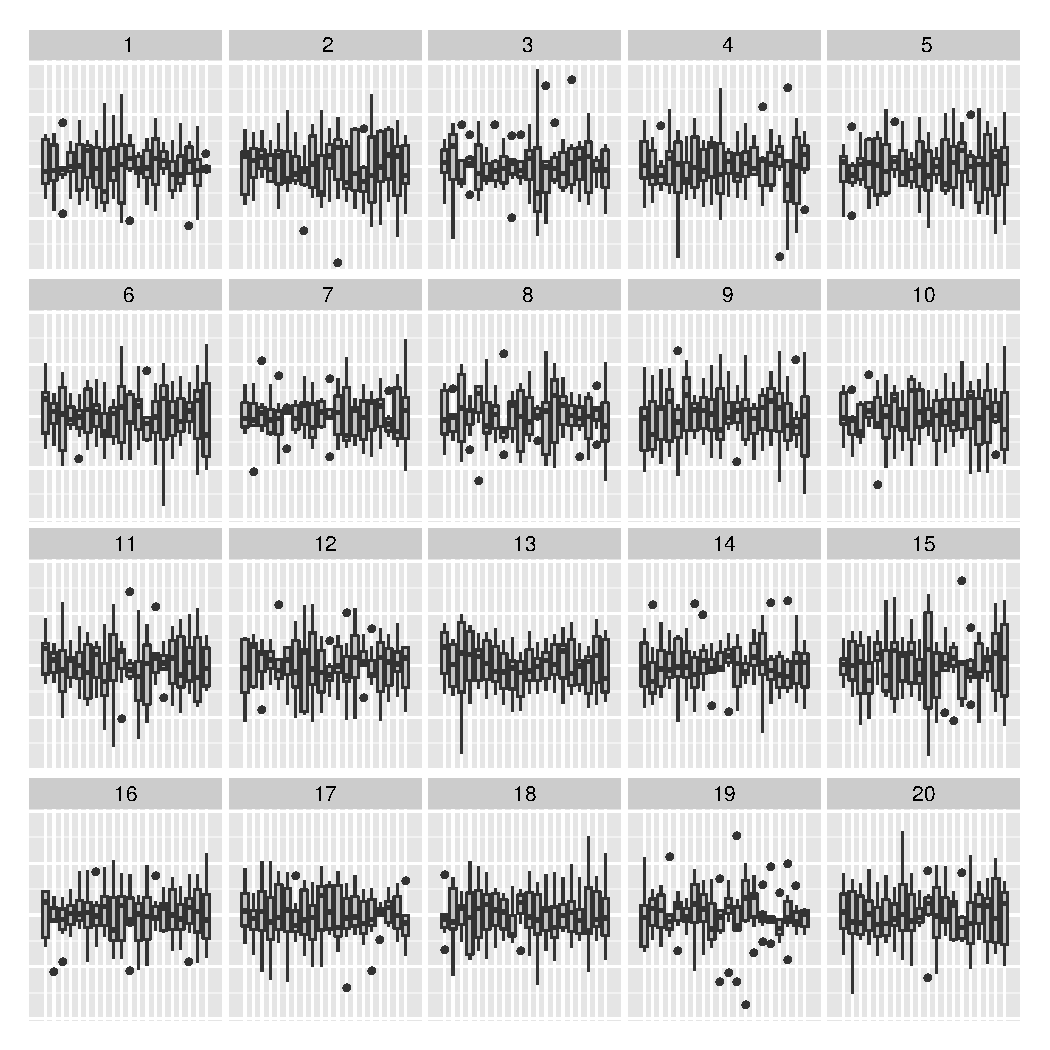
\includegraphics[width=0.8\textwidth]{dialyzerhomogeneous-1-19.pdf}
	\caption{ \label{homogeneous-2}
	Lineup testing homogeneity of the level-1 residuals. Which of the plots is the most different? Which feature led you to your choice?}
%	Lineup of 20 scatterplots of level-1 residuals against pressure used to test the assumption of homogeneous level-1 residual variance for the dialyzer study.  Which is the real plot?}
\end{figure}


%\alnote{Figures~\ref{homogeneous-1} and~\ref{homogeneous-2} are really no different from the cyclone plots, aside from showing two different designs. I am not sure whether they add anything to the discussion in this section. To me they seem to detract from the cyclone plot discussion. One idea is to move them to the appendix where we can highlight the difference in designs. I don't think moving this would detract from how ``novel'' our contribution is.}

Figures~\ref{homogeneous-1} and~\ref{homogeneous-2} show another example of testing for homogeneity in the variance following the approach taken in Section~4.1 of the paper. Both of these lineups are based on the dialyzer data. 
%\alnote{I am confused by plots 7 and 8. What data set are they displaying?}
Level-1 residuals are plotted by subject. Subjects are ordered by variance---i.e.,~we get some structure that might be taken for differences in variability, that are really just differences due to the imbalance in group size. If any panel of this lineup is considered separately, an analyst may come to the conclusion that the within-group variance increases across the $x$ axis.  However, inserting the true plot into the lineup forces the analyst to consider this particular feature as inherent to the data structure rather than evidence against a hypothesis of homogenous variance. 
The dot plot version is not significant, but the box plot version is. When participants in the box plot design identify the data plot, about 45.3\% give outliers as the reason for their choice. In contrast to that, outliers, a large spread or a trend are in a three-way tie for the reason for identifying the data plot in the lineup with the dot plot design.
%Outliers       Large spread       Trend       Asymmetry       Other
% dialyzerhomogeneous
%  correct        1        2        3        4        5
%1   FALSE 38.86852 33.89209 13.35778 12.46726 1.414353
%2    TRUE 25.35211 28.16901 29.57746 16.90141       NA
% dialyzerhomogeneous-bp
%  correct        1        2        3        4        5
%1   FALSE 29.09350 25.72378 28.286664 12.05505 4.841006
%2    TRUE 45.31162 37.28243  8.422235  7.29927 1.684447

The reason for the box plot design being so much more significant might not be so much of an issue of homogeneity being violated as much as a difference in the error distribution between the data and the nulls. Null data come from a parametric bootstrap where residuals are simulated under a normal error assumption. Outliers in small samples are indicative of the sample being from a distribution with heavy tails.
Regardless of the reasoning, the second lineup design enables us to diagnose a problem with the model that makes the data stand out from a set of nulls.  The two designs therefore represent two very similar tests with different power.


%%%%%%%%%%%%%%%%%%%
\clearpage

\bibliographystyle{apalike}
\bibliography{hlmviz_bib}

\end{appendix}

\end{document}